%% LyX 1.6.10 created this file.  For more info, see http://www.lyx.org/.
%% Do not edit unless you really know what you are doing.
\documentclass[english]{article}
\usepackage{lmodern}
\renewcommand{\sfdefault}{lmss}
\usepackage{courier}
\renewcommand{\familydefault}{\rmdefault}
\usepackage[T1]{fontenc}
\usepackage[latin9]{inputenc}
\usepackage{geometry}
\geometry{verbose,tmargin=2cm,bmargin=2cm,lmargin=2cm,rmargin=2cm,headheight=0cm,headsep=0cm,footskip=0cm}
\pagestyle{empty}
\setlength{\parskip}{\smallskipamount}
\setlength{\parindent}{0pt}
\usepackage{graphicx}
\usepackage{setspace}
\onehalfspacing

\makeatletter

%%%%%%%%%%%%%%%%%%%%%%%%%%%%%% LyX specific LaTeX commands.
%% Because html converters don't know tabularnewline
\providecommand{\tabularnewline}{\\}

%%%%%%%%%%%%%%%%%%%%%%%%%%%%%% User specified LaTeX commands.
\makeatother

\makeatother

\usepackage{babel}

\makeatother

\usepackage{babel}

\begin{document}

\title{\textbf{psi46test at DESY}}


\author{Daniel Pitzl, Claudia Seitz, DESY}


\date{23.6.2014}

\maketitle

\section{Introduction}

psi46test is C++ code to test CMS pixel readout chips (ROCs) from
a PC via USB and a pixel test board. It was developed by Beat Meier
at PSI since 2006 to test analog psi46 ROCs with analog ATB test boards.
Functions for digital psi46dig ROCs were added since 2012 and support
for digital DTB test boards started in 2013. The code was developed
under Windows but as plain C++ code without a graphical user interface
it was always running under Linux or on Macintosh as well. The PSI
code is available from git (\texttt{git clone https://github.com/psi46/psi46test.git}).

\noindent The DESY development branched off in March 2014 when DTB
FW/SW version 2.0 appeared. The command line interface is kept. Output
from tests is still written in ASCII format to the log file, but in
addition ROOT histograms are booked, filled, stored, and displayed
in a static canvas. The code is extended with higher level tests for
optimizing DAC settings. The state of the ROC (and the test board)
is represented in software. dacParamter and trimParameter files can
be written in the same format as used by psi46expert and pXar. Code
for the wafer prober at PSI was removed. The code is always tied to
a specific version of the DTB firmware and software (via the RPC remote
procedure call mechanism), which can be inspected at \texttt{https://github.com/psi46/pixel-dtb-firmware)}.
This manual is supposed to document the tests available in the DESY
version of psi46test.


\subsection{Installation}

Install the usb driver library: \texttt{libftd2xx.so} from \texttt{http://www.ftdichip.com/index.html}

A ROOT installation is required (and \texttt{make}, and a C++ compiler).

Install git. Register at \texttt{http://github.com} (invent a user
name and password).

\noindent \texttt{git clone https://user@github.com/clseitz/Psi46testDesy.git}

\texttt{cd Psi46testDesy}

\noindent \texttt{make}

To become a developer (with \texttt{git push} rights) please ask \texttt{Claudia.Seitz@desy.de}
to add your git user name.


\subsection{Start}

Connect a DTB via a USB cable to your computer.

\texttt{cd Psi46test}

\noindent \texttt{bin/psi46test d.log}

You should see something like

\texttt{instantiated a CTestboard}

\texttt{instatiating an iseg HV supply:} (not required)

\texttt{~~unable to open comport: No such file or directory}

\texttt{~~Cannot open COM port}

\texttt{~~cannot open RS232 port} (don't worry)

\texttt{psi46test for DTB V2.2 (4.6.2014)}

\texttt{reading psi46test.ini... }

\texttt{logging to d.log}

(if you get an USB error here that the port cannot be opened on your
computer, \texttt{exit} or \texttt{Ctrl-c} and try\texttt{ . initb.sh}
on Linux)

\texttt{USB opened DTB\_WS6MP2}

\texttt{DTB DTB\_WS6MP2 opened}

(if your output stops here, the DTB firmware may be outdated (before
2.0). You need a psi46test version compatible with any FW from 1.06
to 1.26 and then upgrade dtb\_v2.xy.flash to the current version)

\texttt{-{}-{}- DTB info-{}-{}-{}-{}-{}-{}-{}-{}-{}-{}-{}-{}-{}-{}-{}-{}-{}-{}-{}-{}-{}-{}-{}-{}-{}-{}-{}-{}-{}-{}-{}-{}-{}-{}-{}-{}-}

\texttt{Board id: 77}

\texttt{HW version: DTB1.2}

\texttt{FW version: 2.2}

\texttt{SW version: 2.21}

\texttt{USB id: DTB\_WS6MP2}

\texttt{MAC address: 40D85511804D}

\texttt{Hostname: pixelDTB077}

\texttt{Comment:}

\texttt{-{}-{}-{}-{}-{}-{}-{}-{}-{}-{}-{}-{}-{}-{}-{}-{}-{}-{}-{}-{}-{}-{}-{}-{}-{}-{}-{}-{}-{}-{}-{}-{}-{}-{}-{}-{}-{}-{}-{}-{}-{}-{}-{}-{}-{}-{}-{}-{}-}

\texttt{PC hash 333290928}

\texttt{DTB hash 333290928}

\texttt{RPC call hashes of PC and DTB match: 333290928}

\texttt{ROOT application...}

\texttt{+-cmd commands -{}-{}-{}-{}-{}-{}-{}-{}-{}-{}-{}-{}-{}-{}-{}-{}-{}-{}-{}-{}-{}-+}

\texttt{| help list of commands |}

\texttt{| exit exit commander |}

\texttt{| quit exit commander |}

\texttt{+-{}-{}-{}-{}-{}-{}-{}-{}-{}-{}-{}-{}-{}-{}-{}-{}-{}-{}-{}-{}-{}-{}-{}-{}-{}-{}-{}-{}-{}-{}-{}-{}-{}-{}-{}-+}

\texttt{gainFile: /home/pitzl/psi/dtb/tst215/phroc-c405-trim30.dat}

\texttt{open ROOT window...}

\texttt{MyMainFrame...}

\texttt{open Canvas... }

\texttt{> exit}


\section{commands}

Commands are defined in \texttt{cmd.cpp}. To add a command, put the
code in a new block \texttt{CMD\_PROC(cmdname)\{\}} somewhere in the
file and register it in the \texttt{cmd()} section (towards the end)
with a help string: \texttt{CMD\_REG( cmdname, \textquotedbl{}cmdname
<argument> explain what it does\textquotedbl{} )}. No header files
are involved.

Commands may either be entered interactivley at the prompt, or read
from a file like \texttt{script/mycmd.roc} which gets called from
the prompt by giving the file name without the .roc extension: \texttt{>
mycmd} (the path \texttt{script/} is defined in \texttt{psi46test.ini}).

Commands check for their mandatory arguments and don't execute if
they are missing or out of range. \texttt{help} prints a list of commands
with their parameters.

The state of the ROC (DACs, trims, thresholds) is represented in software.
A test (e.g. a DAC scan) is supposed to restore the original state,
unless a DAC is changed on purpose.

Commands and measurements are written to the log file. This used to
be used for offline parsing, processing, and plotting. It is still
useful for reconstructing the conditions under which a particular
test in a session was executed. Measurements are now also written
as 1D and 2D histograms into a ROOT file \texttt{Test.root}, for direct
plotting and offline processing.


\subsection{DTB commands}

These commands don't require the presence of a ROC. Use them to check
the USB connection and the board. 
\begin{description}
\item [{{{\texttt{rpcinfo}}}}] prints the list of functions available
in the DTB SW via RPC. 
\item [{{\texttt{{upgrade\ dtb\_v2.21.flash}}}}] load new firmware/software
into the FPGA. Wait until the LEDs are off. Exit psi46test. Power
cycle the DTB (unplugging the power cable) to make sure that the new
executable is loaded from EPROM. 
\item [{{{\texttt{help}}}}] prints the list of commands defined in
cmd.cpp 
\item [{{{\texttt{info}}}}] prints DTB info 
\item [{{{\texttt{version}}}}] prints DTB hardware, firmware, and software
version numbers 
\item [{{{\texttt{boardid}}}}] prints the production serial number 
\item [{{{\texttt{welcome}}}}] play the LED startup sequence 
\item [{{{\texttt{setled\ bits}}}}] play with the four LEDs on the
test board (bit pattern: 0 all off, 15 all on) 
\item [{{{\texttt{pon}}}}] low voltage on 
\item [{{{\texttt{getva}}}}] measure the analog supply voltage on the
board 
\item [{{{\texttt{getvd}}}}] measure the digital supply voltage on
the board 
\item [{{{\texttt{va\ mV}}}}] set the analog supply voltage (range
0 to 3000 mV, 1700 mV is fine) 
\item [{{{\texttt{vd\ mV}}}}] set the digital supply voltage (range
0 to 3000 mV, 2500 mV is fine) 
\item [{{{\texttt{poff}}}}] low voltage off. Do this before exiting
from psi46test. 
\item [{{{\texttt{quit}}}}] (or \texttt{exit}) closes the DTB (and
RS232 iseg HV connection, if present), the log and ROOT files and
ends psi46test. 
\end{description}
Rename \texttt{d.log} and/or \texttt{Test.root} if you want to keep
them, otherwise they get overwritten with the next start of \texttt{psi46test}.


\subsection{starting up with a ROC}

Connect a ROC (or module) via adapter board and SCSI cable to the
DTB. You may also want to connect bias voltage (e.g. -150 V) to the
red-ringed lemo connector.

Start again: \texttt{bin/psi46test c405.log} 
\begin{description}
\item [{{{\texttt{s405}}}}] execute start-up commands for a given chip
(\texttt{script/s405.roc}) 
\item [{{{\texttt{getid}}}}] measure digital current, should be around
22-28\,mA per ROC 
\item [{{{\texttt{getia}}}}] measure analog current, should be around
25\,mA per ROC. If it is around 5\,mA the ROC is not properly programmed.
Inspect the settings in the start script. The problem is either here,
or the ROC is dead. 
\item [{{{\texttt{deser160}}}}] 2D scan of clock phase and 160\,MHz
deserializer phase (for single ROCs), searching for the proper ROC
header 7FA (hex). Sets the new values, if successful. 
\end{description}
The following commands elicit a response from the ROC only if it is
properly set up (\texttt{Vana}, \texttt{WBC}, \texttt{CalDel}, \texttt{VthrComp}
are the most critical DACs). See below for more algorithmic procedures. 
\begin{description}
\item [{{{\texttt{fire\ col\ row\ {[}nTrig{]}}}}}] pulse one pixel.
Columns are 0..51, rows are 0..79, default 1 trigger 
\item [{{{\texttt{arm\ col\ row}}}}] enable column, un-mask one pixel
and prepare it for calibrate pulses 
\item [{{{\texttt{arm\ col:col\ row:row}}}}] enable range of columns,
un-mask block of pixels and prepare for calibrate 
\item [{{{\texttt{single}}}}] single calibrate event display (one cycle
of reset-calibrate-trigger-token or whatever is programmed in the
pattern generator) 
\item [{{{\texttt{cole\ col}}}}] enable one column 
\item [{{{\texttt{cole\ col:col}}}}] enable range of columns (e.g.
\texttt{cole 0:51} for all) 
\item [{{{\texttt{pixe\ col\ row}}}}] unmask one pixel 
\item [{{{\texttt{pixe\ col:col\ row:row}}}}] unmask block of pixels
(e.g. \texttt{pixe 0:51 0:79} for the entire ROC) 
\item [{{{\texttt{cal\ col\ row}}}}] activate one pixel for calibrate 
\item [{{{\texttt{cal\ col:col\ row:row}}}}] activate pixels for
calibrate (columns and rows independently, at all intersections of
\texttt{col} and \texttt{row}) 
\item [{{{\texttt{cald}}}}] clear calibrate from all pixels 
\item [{{{\texttt{mask}}}}] disable all pixels 
\item [{{{\texttt{cold\ col}}}}] disable column 
\item [{{{\texttt{pixd\ col\ row}}}}] disable (mask) pixel 
\end{description}

\subsection{DAC parameters}

Table \ref{tab:DACparam} shows the DAC parameters for psi46digV2.1.

%
\begin{table}
\noindent \begin{centering}
\begin{tabular}{|l|l|l|l|l|l|}
\hline 
DAC  & name  & range  & DAC  & name  & range\tabularnewline
\hline
\hline 
1  & Vdig  & 0:15  & 17  & PHOffset  & 0:255\tabularnewline
\hline 
2  & Vana  & 0:255  & 19  & Vcomp\_ADC  & 0:255\tabularnewline
\hline 
3  & Vsf  & 0:255  & 20  & PHScale  & 0:255\tabularnewline
\hline 
4  & Vcomp  & 0:15  & 22  & VIColOr  & 0:255\tabularnewline
\hline 
7  & VwllPr  & 0:255  & 25  & Vcal  & 0:255\tabularnewline
\hline 
9  & VwllSh  & 0:255  & 26  & CalDel  & 0:255\tabularnewline
\hline 
10  & VhldDel  & 0:255  & 253  & CtrlReg  & 0, 4\tabularnewline
\hline 
11  & Vtrim  & 0:255  & 254  & WBC  & 0:255\tabularnewline
\hline 
12  & VthrComp  & 0:255  & 255  & RBreg  & 0:15\tabularnewline
\hline 
13  & VIBias\_Bus  & 0:255  &  &  & \tabularnewline
\hline
\end{tabular}
\par\end{centering}

\protect\caption{DAC paramters for psi46digV2.1\label{tab:DACparam}}
%
\end{table}



\subsection{setting DAC parameters}
\begin{description}
\item [{{{\texttt{optia\ target}}}}] set Vana to get the desired target
analog current {[}mA{]}, .e.g. optia 25 
\item [{{{\texttt{show}}}}] current DAC settings (presumably, from
book-keeping in psi46test; reading back DACs from the ROC is not possible) 
\item [{{{\texttt{dac\ number\ value}}}}] set a DAC value (number
is the DAC address). Some DACs have shortcuts: 
\item [{{{\texttt{vana\ value}}}}] set \texttt{Vana} (check analog
current with \texttt{getia}, 1 mA / 6 Vana DAC units) 
\item [{{{\texttt{vthr\ value}}}}] set global threshold \texttt{VthrComp} 
\item [{{{\texttt{vcal\ value}}}}] set test pulse amplitude 
\item [{{{\texttt{ctl}}}}] set control register (0 = small Vcal, 4
= large Vcal, 1 = ROC off) 
\item [{{{\texttt{caldel\ col\ row}}}}] measure pixel efficiency
vs \texttt{CalDel}, set \texttt{CalDel} in the plateau region 
\item [{{{\texttt{caldelroc}}}}] scan \texttt{CalDel} for the entire
ROC (perfect pixels respond to all triggers, alive pixels have at
least 50\% response), sets \texttt{CalDel} in the plateau region 
\item [{{{\texttt{thrmap\ guess}}}}] measure pixel threshold map for
current settings (faster if guess is close to truth) 
\item [{{{\texttt{vthrcompi}}}}] scan digital current vs global threshold,
set \texttt{VthrComp} below the onset of the noise peak 
\item [{{{\texttt{vthrcomp\ target\,{[}guess{]}}}}}] set VthrComp
such that the minimum pixel threshold is at target Vcal units (faster
if guess is near present threshold) 
\item [{{{\texttt{trim\ target}}}}] set \texttt{Vtrim} and \texttt{trim
bits} such that all pixel thresholds are as close as possible to target
Vcal units 
\item [{{{\texttt{effmap\ nTrig}}}}] measure efficiency map (PixelAlive)
with n triggers per pixel 
\item [{{{\texttt{trimbits}}}}] adjust trim bits to recover maximum
efficiency 
\item [{{{\texttt{wtrim\ chip}}}}] write current trim bits to \texttt{trimParameters\_chip.dat} 
\item [{{{\texttt{phmap\ ntrig}}}}] measure pixel pulse height map 
\item [{{{\texttt{tune}}}}] set gain and offset such that the pulse
heights of all pixels are in 80\% of the ADC range, for large and
small Vcal, with 10\% margins against overflows and underflows 
\item [{{{\texttt{wdac\ chip}}}}] write current DAC settings to \texttt{dacParameters\_chip.dat} 
\end{description}

\subsection{DAC scans}

For diagnostic purposes: scan a dac (or two) for one pixel or the
entire ROC, and measure efficiency, pulse height, or threshold. The
DAC value is restored at the end. 
\begin{description}
\item [{{\texttt{{effdac\ col\ row\ dac}}}}] count trigger responses
(efficiency) for one pixel vs a DAC 
\item [{{\texttt{{phdac\ col\ row\ dac}}}}] pulse height (ADC) vs
DAC for one pixel 
\item [{{{\texttt{calsdac\ col\ row\ dac}}}}] sensor calibrate pulse
height (ADC) vs DAC at CtrlReg 4 (high range Vcal) for one pixel 
\item [{{{\texttt{thrdac\ col\ row\ dac}}}}] threshold (in small
Vcal units) vs DAC for one pixel 
\item [{{{\texttt{dacdac\ col\ row\ dacx\ dacy}}}}] 2D DAC-DAC
scan for one pixel, pulse height and efficiency (26 12 gives the tornado
plot, 26 25 gives the time walk plot) 
\item [{{{\texttt{dacscanroc\ dac\ {[}nTrig{]}}}}}] maps of pulse
height and efficiency vs dac for all pixels (dac 25 at ctl 0 gives
S-curves, dac 25 at ctl 4 gives gain calibration, dac 26 gives CalDel) 
\item [{{{\texttt{gaindac}}}}] calibrated pulse height vs Vcal for
all pixels, checks the gain calibration 
\end{description}

\subsection{maps}
\begin{description}
\item [{{{\texttt{effmap\ nTrig}}}}] pixel efficiency map (PixelAlive) 
\item [{{{\texttt{thrmap\ guess}}}}] measure pixel threshold map for
current settings (faster if guess is close to truth) 
\item [{{{\texttt{phmap\ nTrig}}}}] pulse height map (vary \texttt{vcal}
and \texttt{ctl} to explore the full range) 
\end{description}

\subsection{sensor calibrate and bump bond test}

The ROC test pulse may be directed towards a pad on the surface of
each pixel, inducing a (small) charge into the sensor across the air
gap capacitance, which can be detected if the bump bond connection
is good.

The tests internally select \texttt{ctl 4} to get the large test pulse
range (and set it back to previous). 
\begin{description}
\item [{{{\texttt{cals\ col\ row}}}}] active one pixel for sensor
calibrate (requires \texttt{cole col }and\texttt{ pixe col row} to
see the response with \texttt{single}) 
\item [{{{\texttt{calsdac\ col\ row\ dac}}}}] sensor calibrate pulse
height (ADC) vs DAC at CtrlReg 4 (high range Vcal) for one pixel 
\item [{{{\texttt{calsmap\ nTrig}}}}] sensor calibrate pulse height
map 
\item [{{{\texttt{bbtest\ nTrig}}}}] sensor calibrate pulse height
map with bump bond statistics 
\item [{{{\texttt{dacscanroc\ dac\ -nTrig}}}}] sensor calibrate (selected
by negative nTrig) pulse height and efficiency vs dac for all pixels
(\texttt{dac} 12 at \texttt{ctl} 4 gives bump bond test) 
\end{description}

\subsection{data taking}

The pattern generator on the DTB can be operated in a loop, repeating
its programmed cycle (typically reset-cal-trigger-token = rctk) at
an adjustable rate. The rate is determined by the clock frequency
(typically 40\,MHz) and the sum of the delays in the pattern generator
sequence (at least WBC) plus a programmable delay: R = f / N, e.g. 
\begin{description}
\item [{{{\texttt{pgloop\ 1000}}}}] gives a rate of about 40\,kHz. 
\end{description}
A DAQ process is started on the DTB such that the FPGA writes the
deserialized raw data into memory. Up to 50 M words (100\,MB) can
be stored. The pattern generator loop and the DAQ are stopped every
few ms and the memory is readout via USB. This introdcues some dead
time but allows for almost concurrent decoding and display of the
data.

The result are random trigger hit maps and pulse height distributions,
which can be used with sources (X-ray, Sr, Ru), with fixed test pulse
patterns (arm), or just with noise (at lowest thresholds, enable all
pixels).


\section{algorithms}

Details about algorithms that set DAC parameters.


\subsection{analog current}

DAC \texttt{Vana} controls the analog current that supplies pre-ampliefer
and shaper of each pixel. The current is measured on the test board
(\texttt{getia}). There is an offset current of about 5\,mA per ROC
for \texttt{Vana} = 0. At full range (\texttt{Vana} 255) the current
is about 45\,mA per ROC, with an approximately linear dependence
and a slope of 1\,mA / 6 DAC units. The design operating analog current
is 24\,mA / ROC. Command \texttt{optia target} takes the desired
current {[}mA{]} as an argument and tries to adjust \texttt{Vana}
accordingly. It usually succeeds in a few iterations.


\subsection{timing}

Coarse (unit: BC = clock cycles = 25\,ns): \texttt{WBC = tct\,-\,7}
for psi46digV2.1, \texttt{WBC = tct\,-\,6} for earlier digital ROCs,
\texttt{WBC = tct\,-\,5} for analog ROCs, where \texttt{tct} ist
the time between calibrate and trigger in the pattern generator sequence
(e.g. \texttt{WBC 99} for \texttt{tct 106}).

Fine: \texttt{CalDel} shifts the timing of the test pulse, unit: 1\,DAC
\ensuremath{\approx} 0.4\,ns, dynamic range 0..255 \ensuremath{\approx}
100\,ns = 4\,BC.


\subsection{threshold trimming}

Symbolic equation: pixelThreshold = globalThreshold - \texttt{Vtrim\,(15\,-\,trim
bits)}, where the pixel threshold is determined from a Vcal scan with
several triggers per point, searching for the point of 50\% response.
In low Vcal range (CtrlReg 0), a Vcal threshold of 30 DAC units corresponds
to about 1500 electrons signal. \texttt{VthrComp} and \texttt{Vtrim}
are global DACs, affecting the entire ROC, while the four \texttt{trim
bits} can be set for each pixel individually. As the equation shows,
the trimming can only lower the threshold from the value determined
by \texttt{VthrComp}. The \texttt{trim bits} act inverted: 15 means
no effect, while 0 gives the maximum threshold reduction as allowed
by \texttt{Vtrim}. Due to transistor variations from pixel to pixel
the untrimmed threshold distribution (Vtrim 0, trim bits 15) is rather
broad, with an RMS of typically 6 Vcal DAC units and a non-Gaussian
distribution that reflects geographical variations across the ROC.
The goal of the trimming procedure is to sharpen the threshold distribution
to about 1 Vcal DAC unit (50 e) and a mean value a low as possible,
but staying clear by at least 6\,$\sigma$ from the noise level.
The dynamic range of the threshold DACs is rather large (except for
digV2 ROCs at nominal analog current), so that thresholds from 1\,ke
to 10\,ke can be reached, in 50\,e steps. The trimming procedure
thus starts with selecting a threshold target (e.g. 30 Vcal DAC units),
and adjusting the DACs and bits to reach that. A second constraint
can be derived from the threshold equation: a smaller value of Vtrim
leads to a closer spacing of the trim bit steps and a sharper threshold
distribution.

The trimming procedure starts by measuring the untrimmed threshold
distribution and identifying one pixel with the highest and one with
the lowest threshold (dead pixels are flagged and ignored).


\subsubsection{Global threshold}

\texttt{VthrComp} acts inversely: a smaller DAC setting gives a harder
globalThreshold (higher in Vcal DAC units). VthrComp is determined
from the lowest pixel in the untrimmed distribution, setting its threshold
to the target value (and pulling all other pixels along): command
\texttt{vthrcomp} target.

Changing the threshold may influence the timing of the comparator,
so CalDel should be checked and adjusted (command \texttt{caldelroc}).


\subsubsection{Vtrim}

The pixel with the highest threshold in the untrimmed distribution
is used to set Vtrim, since it needs the largest correction. Its trim
bits are set to 0 for maximum effect and Vtrim is increased until
the target threshold is reached (command \texttt{trim target})


\subsubsection{trim bits}

The trim bits are set in five iterations in the same trim command.
First, all trim bits are set to 7 (half way) and a threshold map is
taken. Many pixels may already be in the noise and don't respond;
this is recognized and their trim bits are increased again in subsequent
steps. For the others, the measured threshold is compared to the target,
and the trim bits are adjusted in steps of 4, 2, 1, and 1 units, with
the appropriate sign. A final threshold map should be taken for documentation
(command \texttt{thrmap guess}, where \texttt{target} is a good guess).


\subsubsection{efficiency check}

The trimming procedure requires only 50\% response for a valid threshold
measurement. Some pixels apparently end up too close to the noise
and require some further trim bit adjustment. An efficiency map with
e.g. 100 triggers per pixel is taken and all pixels below 100\% are
inspected. Their trim bits are increased in steps of one until 100\%
response or end of range at 15 is reached (command \texttt{trimbits}).

The trim bits can be written to an ASCII file (\texttt{trimParameters\_chip.dat})
with the comand \texttt{wtrim chip}.


\subsection{pulse height tuning}

Adjust gain and offset such that all pixel pulse heights fit into
the 8 bit ADC range, for large and small Vcal. Leaving a safety margin
of 22 ADC units at the top and 33 units at the bottom the available
range is about 200 ADC counts. One pulse height ADC count then corresponds
to 150 e charge, which is equal to the single pixel noise and the
resolution loss due to digitization is smaller.

Starting from default gain and offset parameters, several pixel may
be in ADC overflow or underflow. Here we use a trick taken from some
ETH code: setting the gain DAC to minimum usually brings all pixels
into the ADC range, with small spread, so a single test pixel is enough.
Use the offset DAC to set this pulse height in the middle of the ADC
range. Increase the gain until the top or bottom safety margin is
reached. Take pulse height maps at largest Vcal and close to threshold.
Find the pixels with maximum large and minimum small response. Use
these two pixels for final adjustment of gain and offset within the
safety margins.

It is best to do pulse height tuning after threshold trimming to explore
the low Vcal range. 
\begin{description}
\item [{{tune~col~row}}] pulse height tuning procedure using the given
pixel for the first steps. Sets gain and offset DACs. 
\item [{{phmap~nTrig}}] take pulse height maps at large and small Vcal
to verify te result. 
\end{description}
The DACs used for offset and gain depend on the digital ROC version:
for psi46dig and digV2 we use \texttt{VoffsetOp} (15) and \texttt{VIref\_ADC}
(20), while for psi46digV2.1 we use \texttt{PHOffset} (17) and \texttt{PHScale}
(20).


\section{offline processing}

The ROOT and log files from some tests can be used for further processing
and analysis, typically in ROOT.


\subsection{gain calibration\label{sub:gaincalib}}

Pulse height gain and offset varies from pixel to pixel. For best
position resolution (using charge information) the variation should
be calibrated out (can we quantify this? test beam analysis with the
raw pulse height!). The calibrated pulse height distributions allow
monitoring of the threshold and of the sensor charge collection efficiency
in beam data.

The gain calibration starts from scans of pulse height vs test pulse
amplitude, in low and high range: 
\begin{description}
\item [{{{\texttt{ctl\ 0}}}}] small Vcal 
\item [{{{\texttt{dacscanroc\ 25\ nTrig}}}}] measure pulse height
vs Vcal for each pixel, nTrig = 10 takes about 90 s, filling a 2D
histogram \texttt{PH\_DAC25\_CR0\_map} 
\item [{{{\texttt{ctl\ 4}}}}] large Vcal 
\item [{{{\texttt{dacscanroc\ 25\ nTrig}}}}] filling \texttt{TH2D
PH\_DAC25\_CR4\_map} 
\end{description}
\texttt{mv Test.root phroc-c405-Ia25-trim30.root}

The gain calibration varies with several dacs (Vdig, Vana, Vsf, Vrg,
Vtrim, VthrComp, PHOffset, PHscale) and with temperature.

It was found that the gain curve (PH vs Vcal) of digital ROCs is well
described by a Weibull distribution function:

\[
f=p_{4}-p_{3}\exp(-t^{p_{2}}),\: t=p_{0}+x/p_{1}\]


where x is the test pulse amplitude (Vcal DAC) and f the measured
pulse height {[}ADC{]}. $p_{4}$ is the asymptotic pulse height (in
the saturation region), $p_{3}$ is the dynamic range from zero to
saturation and the rest are shape parameters which can be given an
interpretation by looking at the derivatives:

\[
f'=p_{3}p_{2}t^{p_{2}-1}\exp(-t^{p_{2}})/p_{1},\: f''=-p_{3}p_{2}\exp(-t^{p_{2}})\left((p_{2}-1)t^{p_{2}-2}-p_{2}t^{p_{2}-1}\right)/p_{1}^{2}\]


$f$ has an inflection point where $f'$ has a maximum and where $f''$
has a zero, namely at $t_{inf}=\left((p_{2}-1)/p_{2}\right)^{1/p_{2}}$.
The maximum gain is then $f'(t_{inf})$.

It turns out that $p_{0}$ is always very close to one (like 0.9998).
It is thus tempting to reduce the number of parameters by setting
$p_{0}$ to one. Furthermore, $p_{1}$ turns out to be rather large
($10^{5}$ in Vcal DAC units), inviting one more approximation:

\[
t^{p_{2}}\approx\left(1+x/p_{1}\right)^{p_{2}}=\exp\left(p_{2}\ln(1+x/p_{1})\right)\approx\exp\left(p_{2}x/p_{1}\right)\]


leading to a double exponential

\[
f\approx p_{4}-p_{3}\exp\left(-\exp(p_{2}x/p_{1})\right)\]


which is known as the Gompertz function. It describes the transition
towards saturation quite well but has slope zero at $x=0$ while the
gain curve rises almost linearly from threshold. We use the Weibull
fit (the $\tanh$ fit used for analog ROCs does not give a good discription
of the turn-over towards saturation; it is too sharp).

The fit is done simultaneously to the low Vcal ($x_{0}$) and high
Vcal($x_{4}$) range measurements using one more parameter for rescaling
Vcal: $x_{0}=x_{4}/p_{5}$, where $p_{5}$ is around 7.

The fit is numerically problematic as not only do the parameter values
range over several orders of magnitude (which could be cured by rescaling)
but also their precisions. This is reflected in a huge condition number
($10^{16}$) for the Hessian matrix (which upon convergence is the
inverse of the covariance matrix of the fit parameters). Convergence
depends crucially on the start values for the parameters. However,
we want to perform $10^{8}$fits automatically but successfully. Migrad
(from Minuit) may converge for 95\% to 99\% of the pixels which is
not good enough. A modern quadratic approximation optimization algorithm
(BObyQA) or gradient based algorithms (the derivatives of $f$ with
respect the parameters $p_{i}$ are analytic) like L-BFGS do not fare
better. The best performance was found with the good old Nelder-Mead
simplex algorithm, which reaches 100\% convergence and finds the same
$\chi^{2}$ minimum as the other algorithms in the cases where they
all converge.

In data analysis, and also for gain monitoring in psi46test, the inverse
function is needed to translate a measured pulse height $a$ from
ADC counts into Vcal DAC units:

\[
f^{-1}=p_{1}\left(\left(-\ln\left((p_{4}-a)/p_{3}\right)\right)^{1/p_{2}}-p_{0}\right)\]


which is nicely analytic but reveals one problem: the argument of
the logarithm must be positive, thus the measured pulse height $a$
must never fluctuate above the asymptotic value $p_{4}$. A protection
is put in place, leading to an artificial peak at large pulse heights
(but reflecting the loss of pulse height sensitivity in the saturation
region).


\subsection{S-curves}

S-curve is descriptive pixel slang for threshold curves as obtained
from counting the number of pixel responses to a given number of triggers
$N$ as a function of a dac. Each response count $n_{i}$ is drawn
from a binomial distribution with unknown success probability. The
fit involves a model for the success probability as a function of
the dac. When the width of the threshold is governed by noise, a Gaussian
error distribution ranging from 0 to 100\% is well justified. In the
presence of non-Gaussian tails one may try a Student's $t$ distribution.
A general threshold can often be parametrized by a Fermi function
(which is equivalent to a $\tanh$ function). In all cases, the quoted
threshold is defined as the dac value where 50\% efficiency is reached.
In this way, the threshold can also be determined without fitting,
just by scanning the data curve, as is done in the FPGA. The width
of the S-curve can be determined from the 10\% to 90\% range, which
is $2.56\,\sigma$ for the Gaussian error distribution. If the gain
calibration from Section \ref{sub:gaincalib} was executed beforehand
one can use the outputfile that was already produced (for small pulses
ctl 0), otherwise do: 
\begin{description}
\item [{{{ctl\ 0}}}] Test should be done with small Vcal 
\item [{{{dacscanroc\ 25\ nTrig}}}] fills TH2D histograms for puls
height (\texttt{PH\_DAC25\_CR0\_map}) and number of reponses (\texttt{N\_DAC25\_CR0\_map}),
S-curves are determined from the number of responses 
\end{description}
\texttt{mv Test.root scurves-c405-trim30.root}

A script exists to analyze this root file, extract the number of responses
histogram for each pixel, and perform a fit to the distribution as
shown in Figure.

%
\begin{figure}
\noindent \begin{centering}
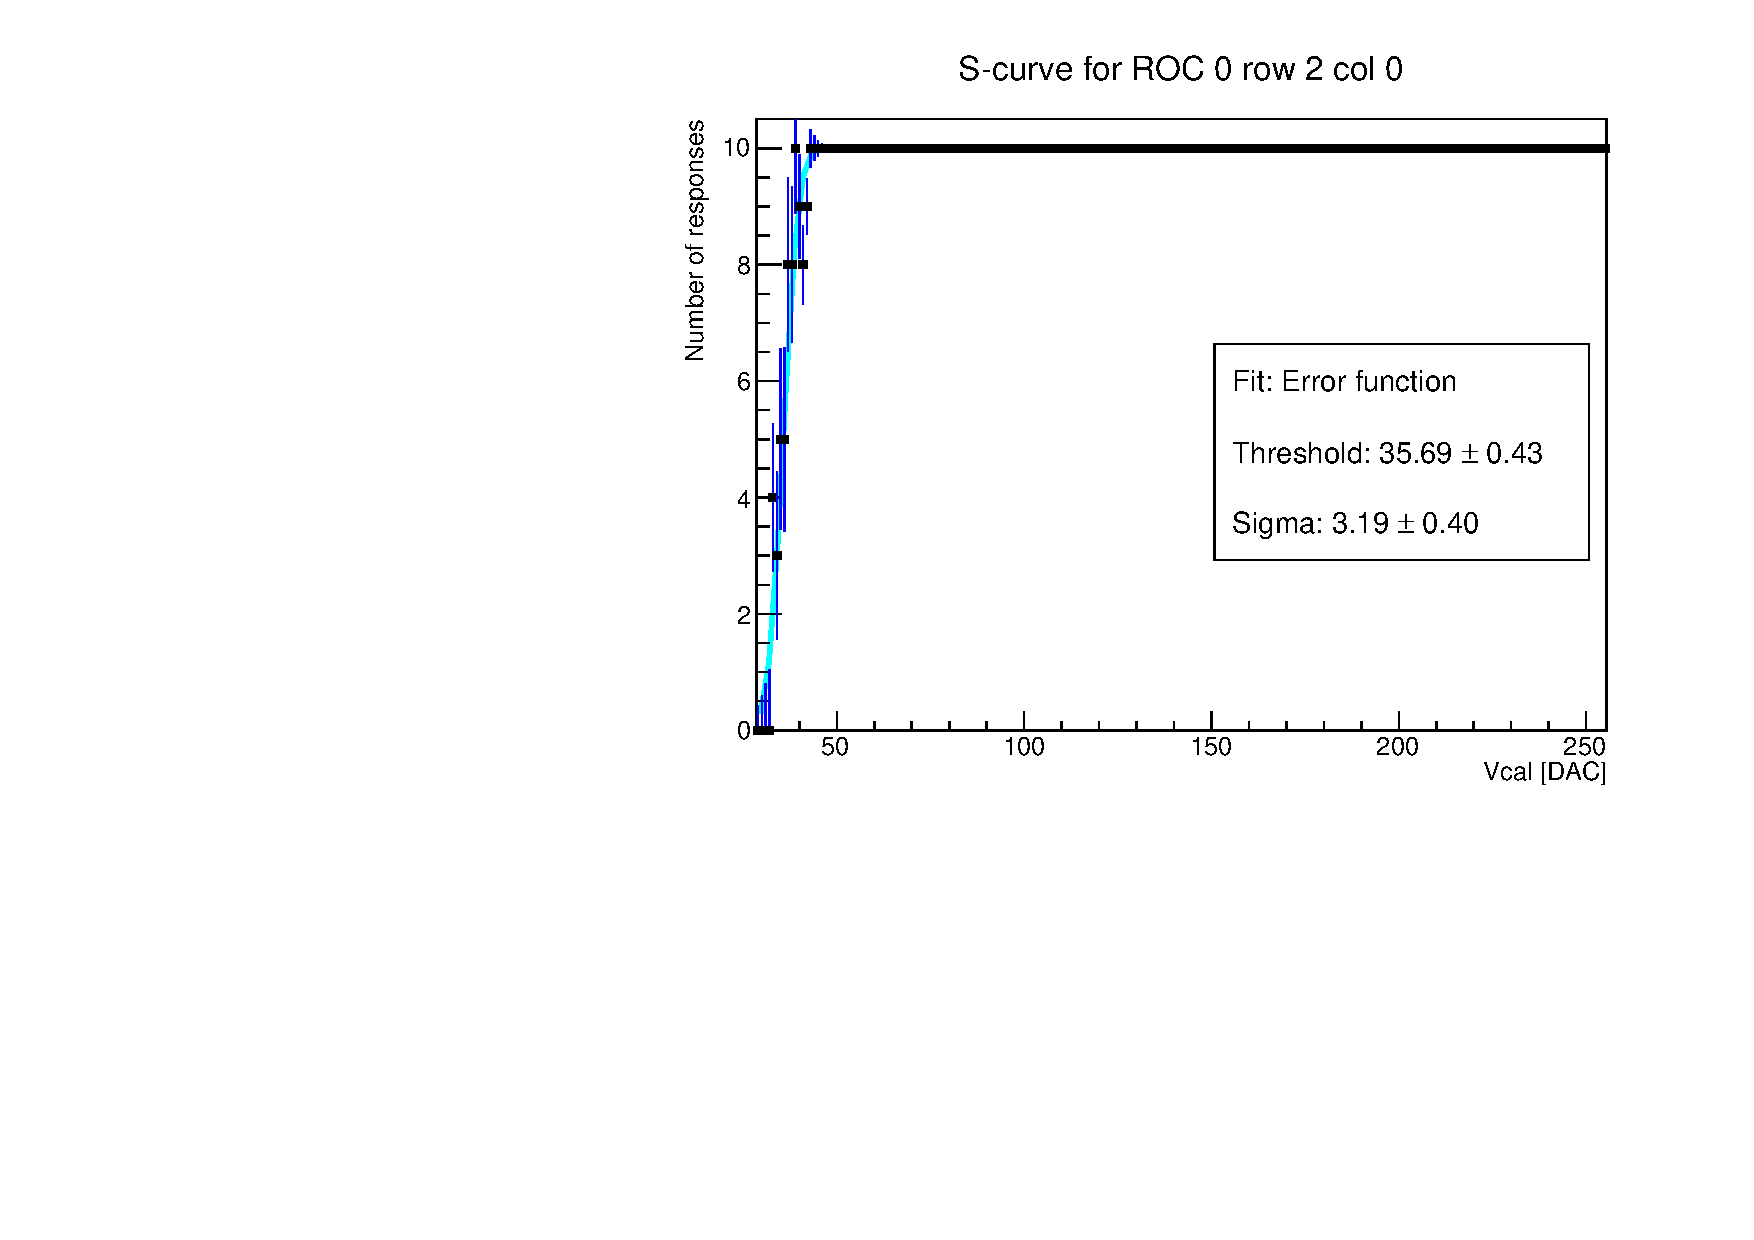
\includegraphics[scale=0.5]{c405-thrdist-scurve-trim36} 
\par\end{centering}

\protect\caption{Distribution of the number of responses as a function of Vcal fitted
with an Error function for one pixel.}
%
\end{figure}


This plot is produced and a root tree is written out that can be used
for further analysis.

\texttt{root -l scurves-c405-trim30.root}

\texttt{.x ROCscurve\_fit.C+}

This will run for a bit and produce two output files: minscurves.ps
(containing all the s-curve plots/fits for each pixel) and fit\_results\_scurve\_\{originalname\}.root
(containing a tree with threshold, sigma, fit stauts, and chisquare
for each pixel).

The tree output file can be further analyzed with the following macro:

\texttt{root -l fit\_results\_\{originalname\}.root}

\texttt{.x ROCscurve\_ana.C}

This creates the threshold and sigma distribution for all the pixels,
as well as maps showing the threshold and sigma for each pixel and
saves them in threshold\_scurve.ps.

%
\begin{figure}
\noindent \begin{centering}
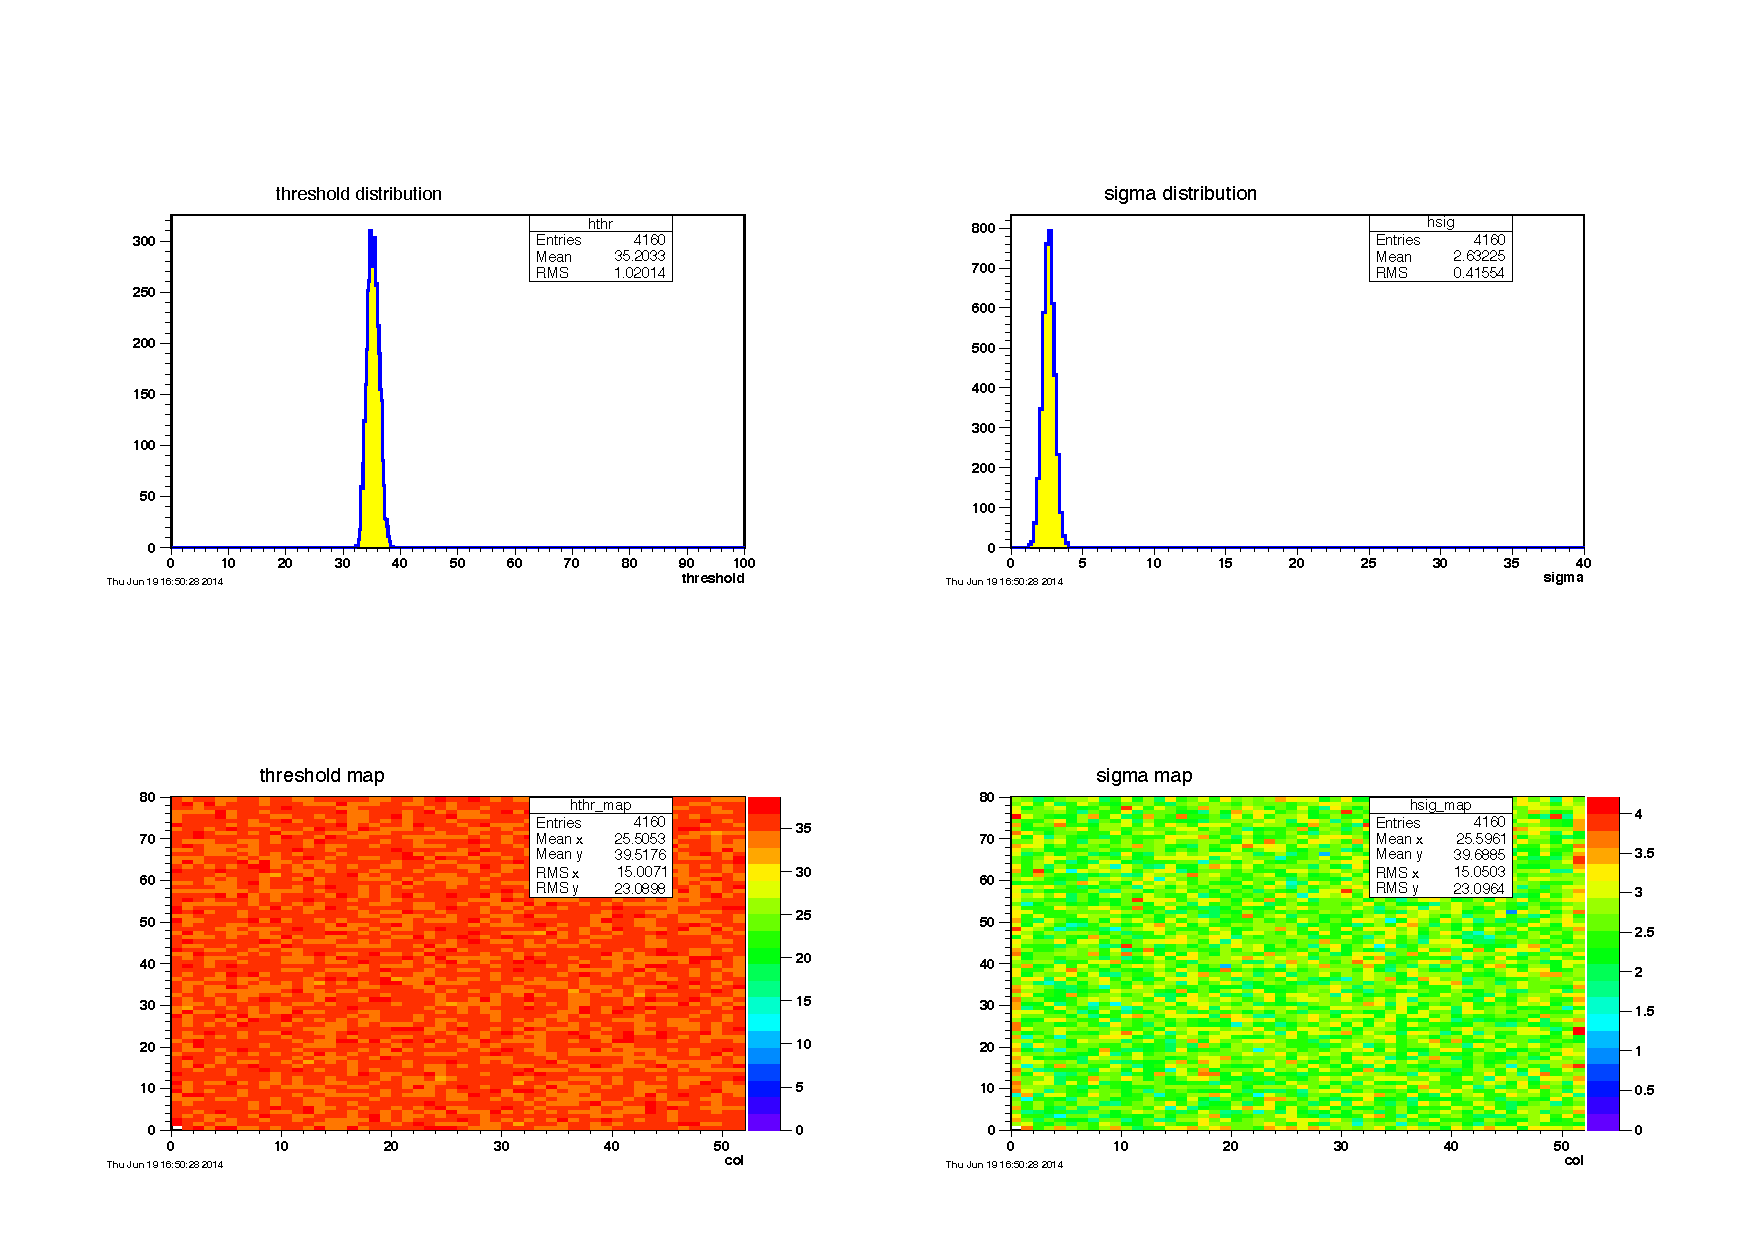
\includegraphics[scale=0.6]{c405-thrsigma-trim36} 
\par\end{centering}

\protect\caption{The top row shows the threshold distribution (left) and the width
(sigma) of the error function (right) for all pixels on a ROC. The
bottom row shows the threshold map (left) and sigma map (right) for
all pixels.}
%
\end{figure}



\subsection{bump bond test}

The ROC has a switch (\texttt{cals}) on each pixel which allows to
send the test pulse to a pad on the top metal layer. When a sensor
is present it forms a (small) air gap capacitance and some charge
gets induced. When the bump bond is functional the pixel circuit amplifies
the signal and if the threshold is sufficiently low it can be detected
and read out. Two tests are available: 
\begin{description}
\item [{{{\texttt{bbtest\ nTrig}}}}] fast map of all pixels' responses
to \texttt{cals} pulses, done with the largest pulse (\texttt{CtrlReg}
4, \texttt{Vcal} 255) but with fixed threshold settings. 
\item [{{{\texttt{dacscanroc\ 12\ -nTrig}}}}] scan global threshold
\texttt{VthrComp} while pulsing through the sensor (selected with
negative nTrig). Should be done with large pulses (\texttt{CtrlReg}
4, \texttt{Vcal} 255). 
\end{description}
\clearpage{}


\section{plots}

%
\begin{figure}
\hfill{}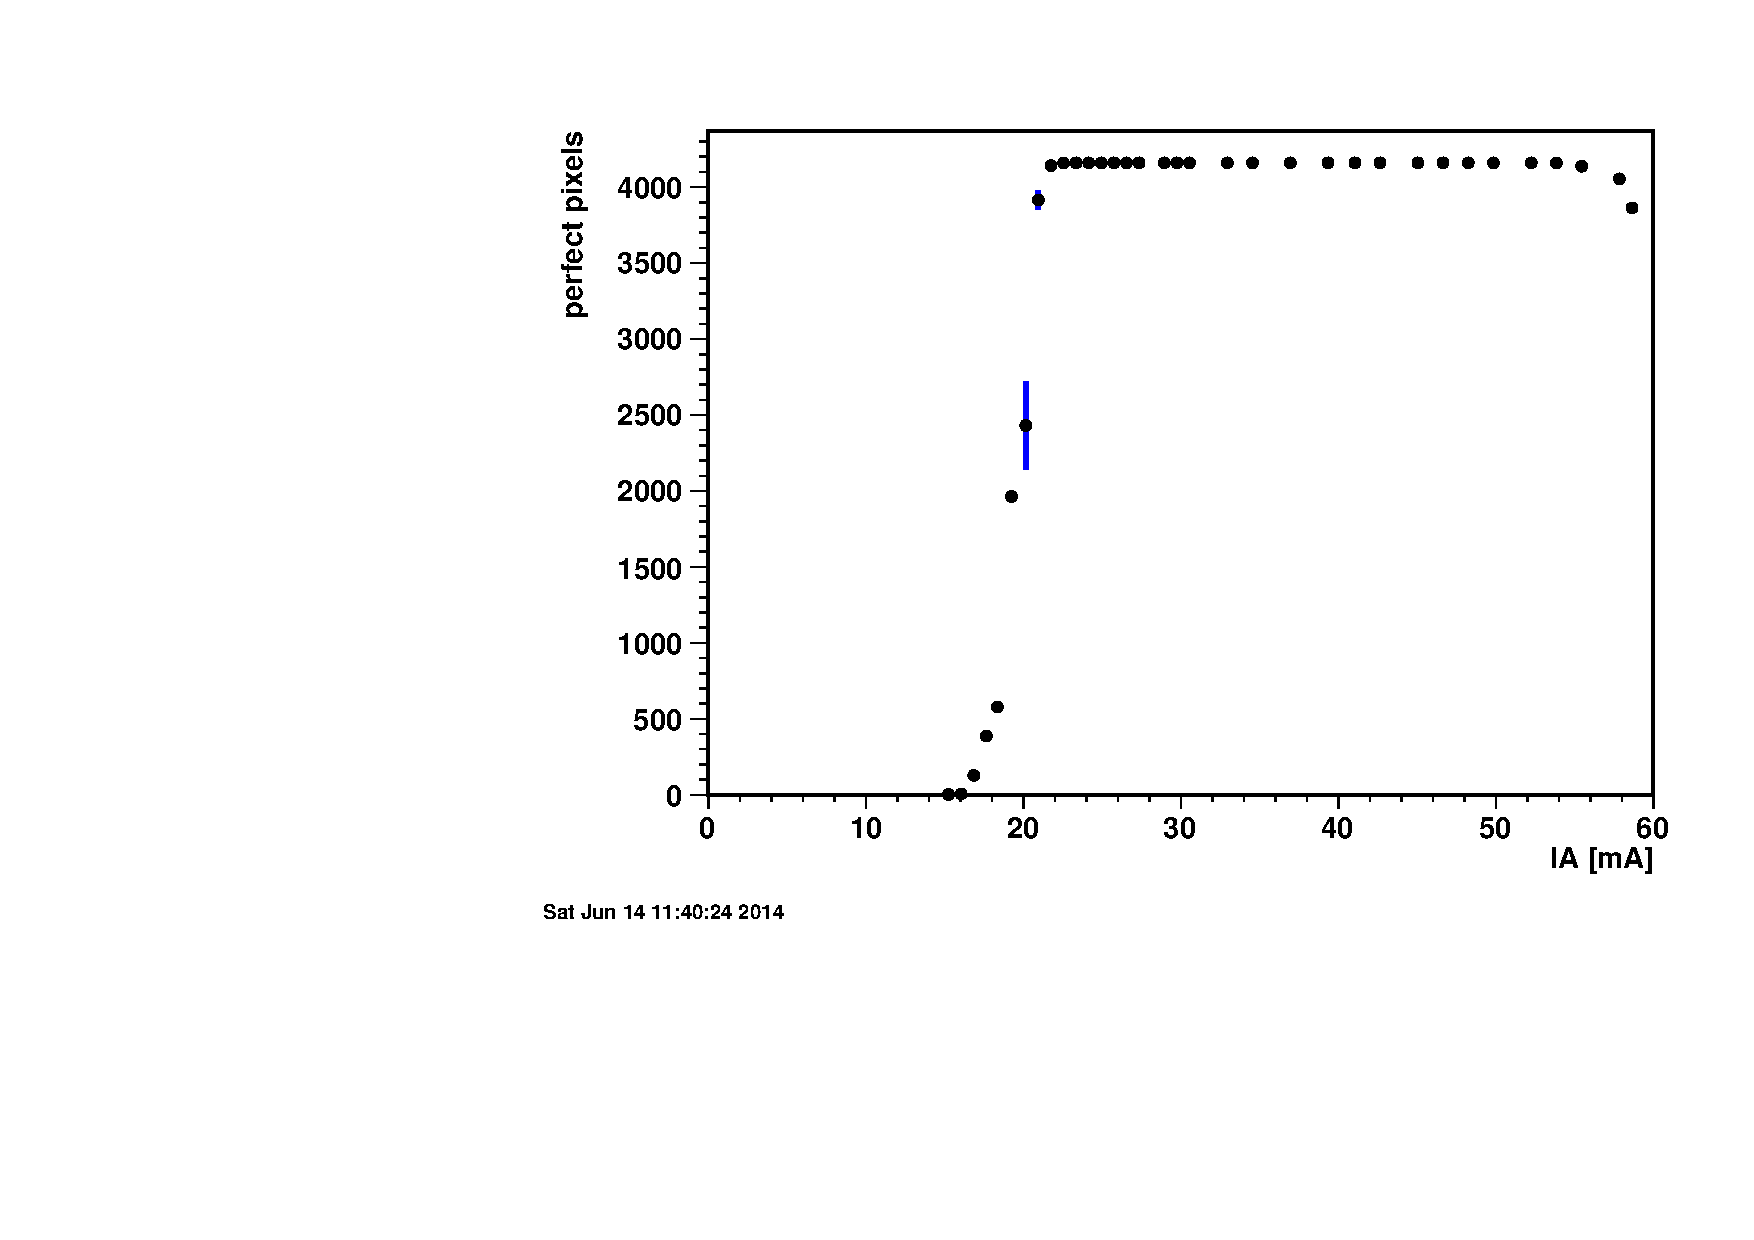
\includegraphics[scale=0.5]{c405-perfect-va-Ia}\hfill{}~\protect\caption{perfectly efficient pixels vs analog current. 22\,mA is required
to reach the plateau. At large current the effective threshold is
too high}
%
\end{figure}


%
\begin{figure}[h]
 \hfill{}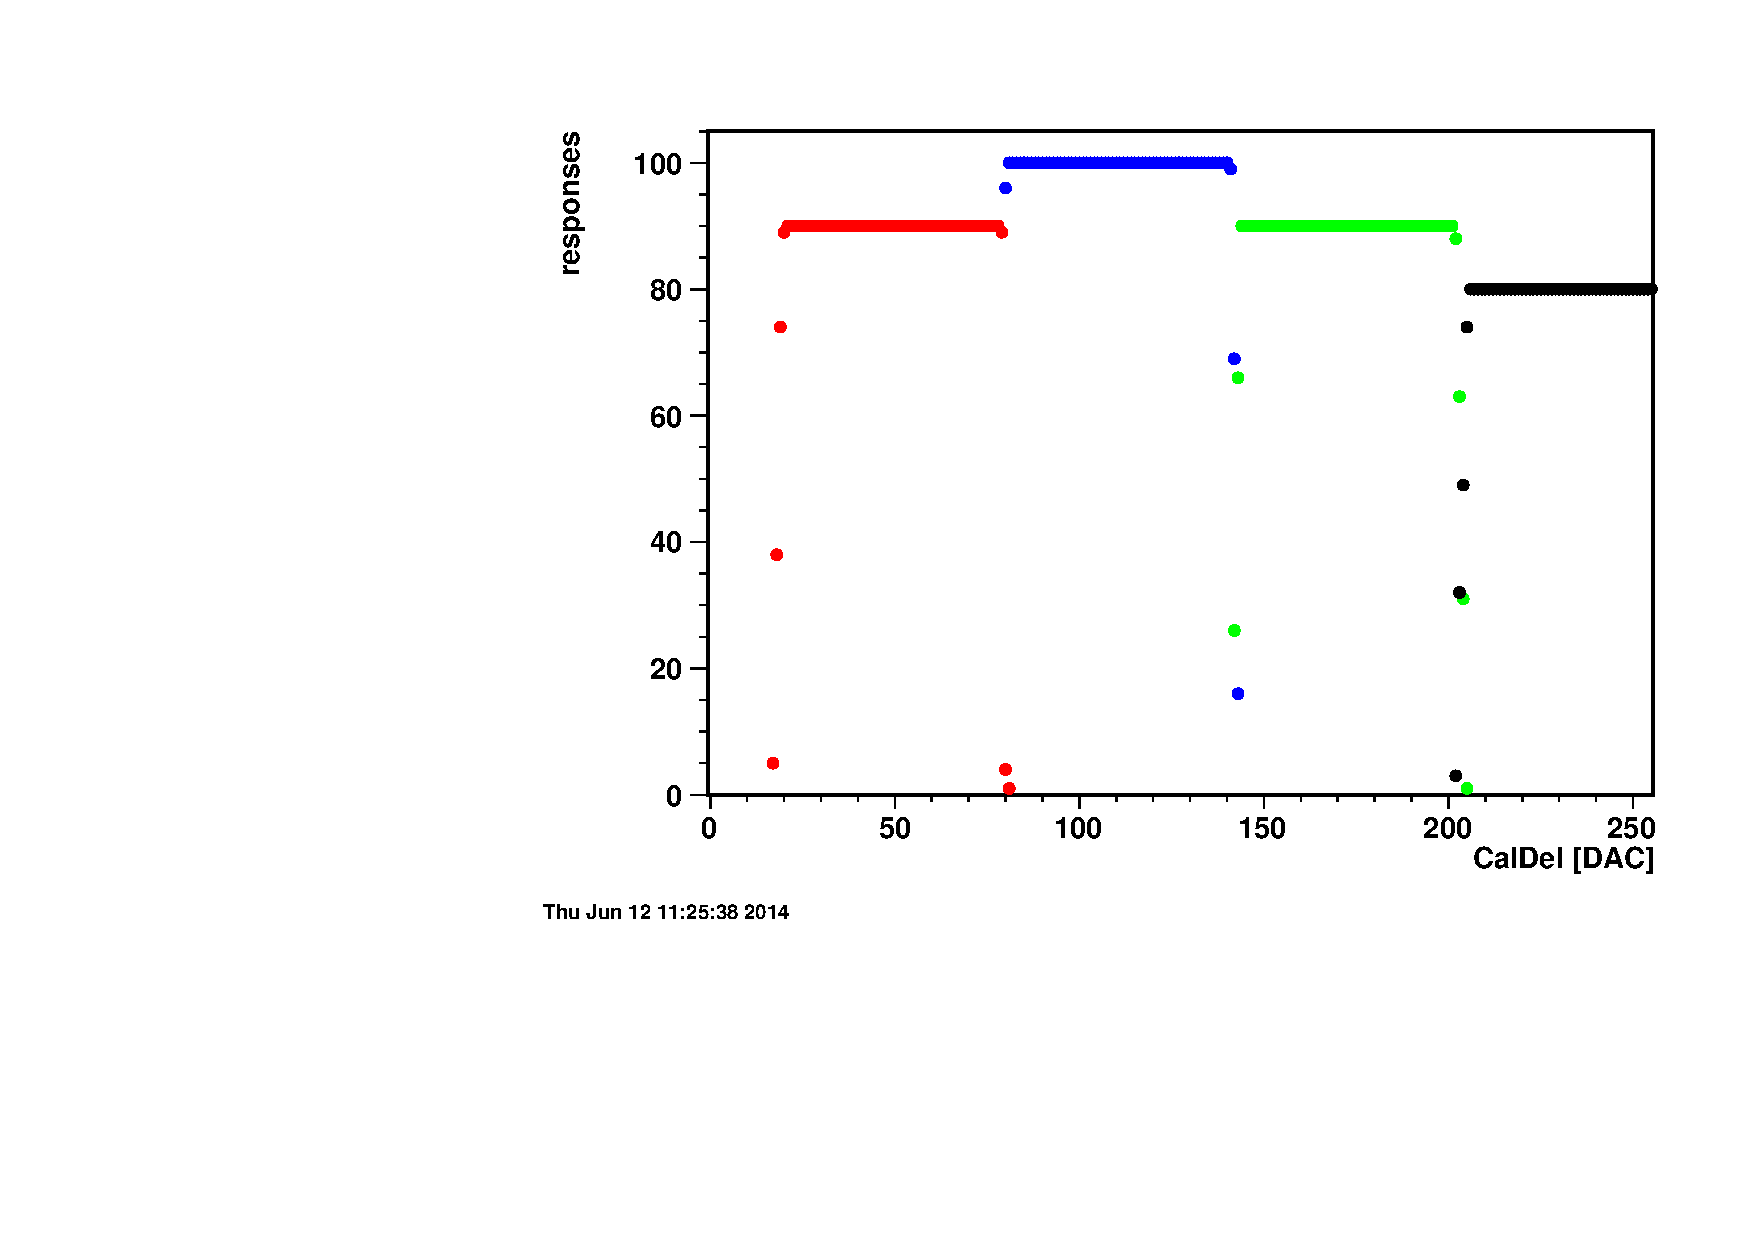
\includegraphics[bb=0bp 0bp 567bp 480bp,scale=0.66]{c405-caldel-wbc-97-98-99-100}\hfill{}~

\protect\caption{Responses vs \texttt{CalDel} for one pixel. tct 106. \texttt{WBC}
100 (red, 90 triggers), \texttt{WBC} 99 (blue, 100 triggers, working
point), \texttt{WBC} 98 (green, 90 triggers), \texttt{WBC} 97 (black,
80 triggers).}
%
\end{figure}


%
\begin{figure}[h]
 \hfill{}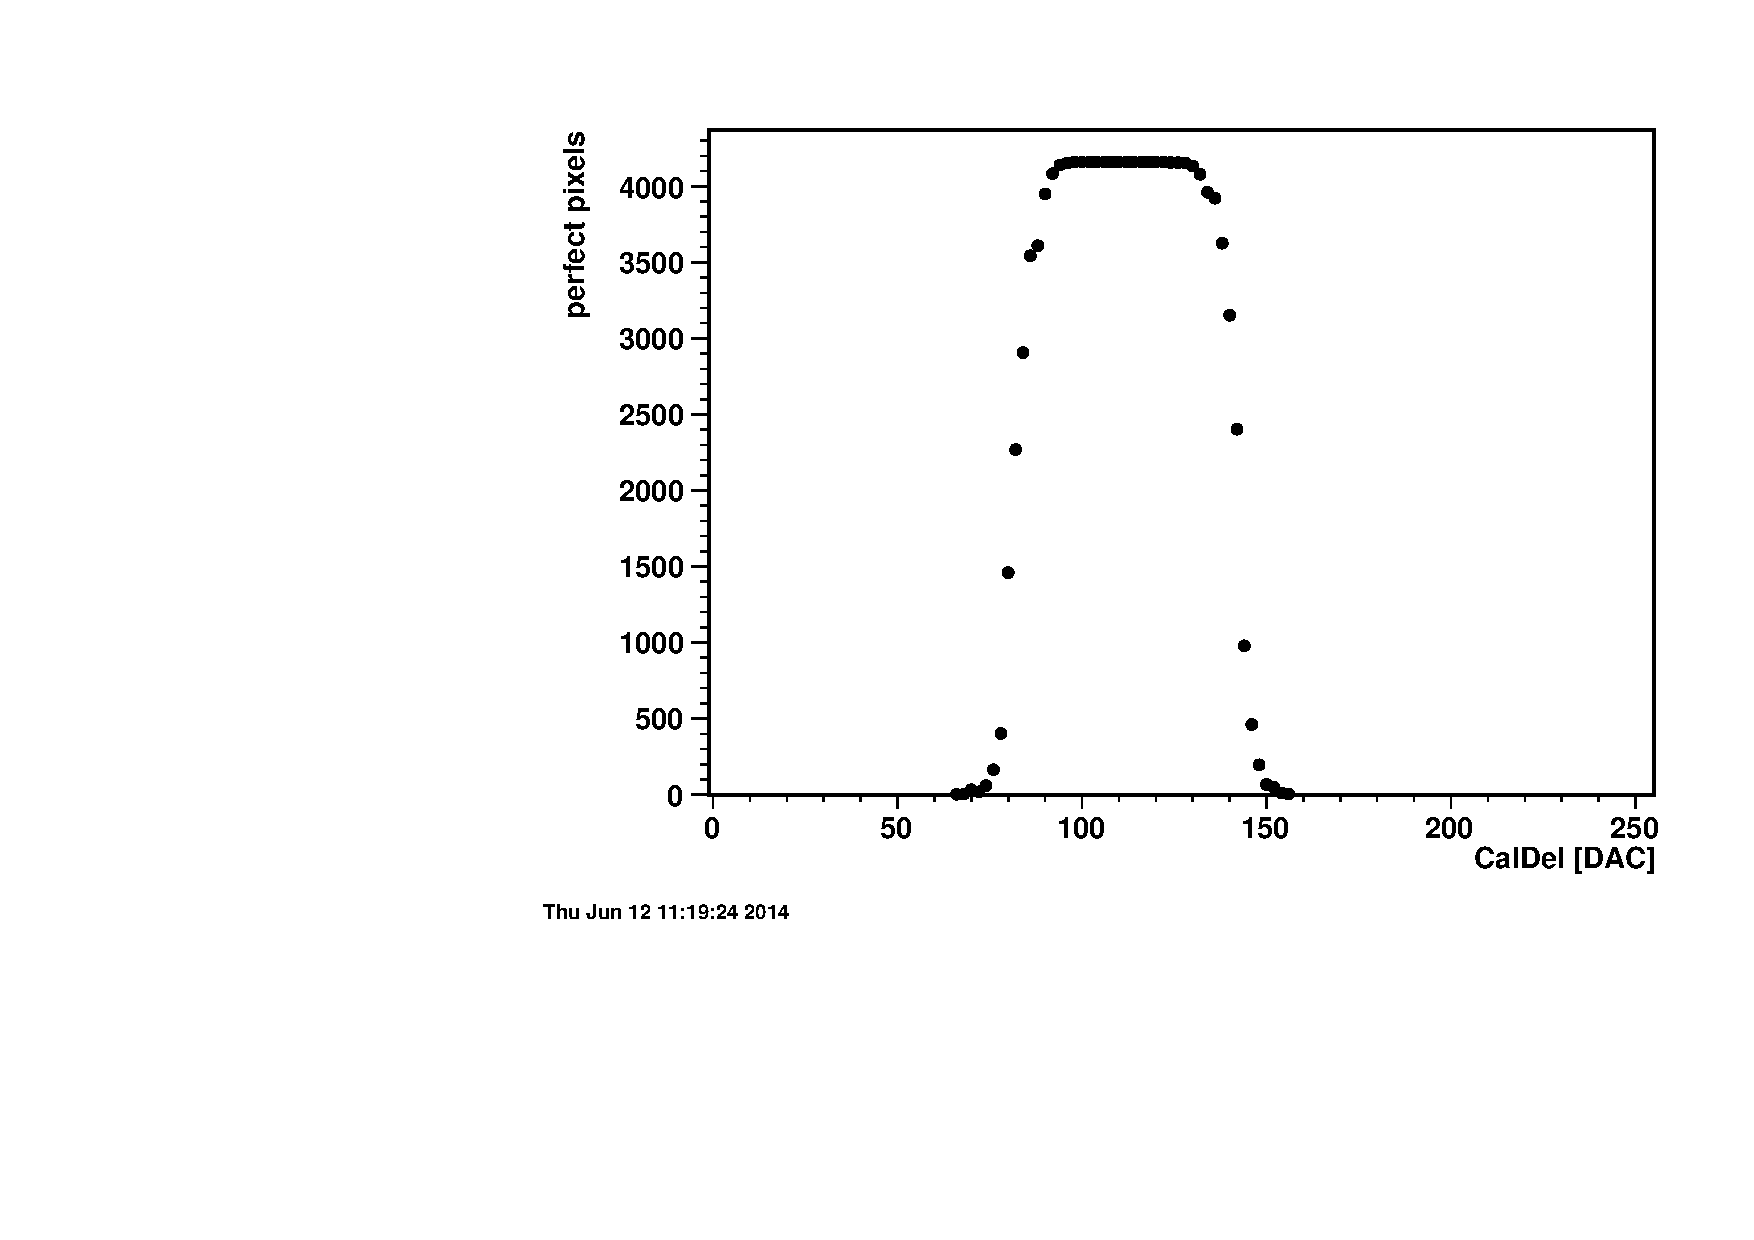
\includegraphics[bb=0bp 0bp 567bp 425bp,scale=0.5]{c405-caldelroc}\hfill{}~\protect\caption{\texttt{CalDel} scan for an entire ROC counting the number of fully
responding pixels at each point at large \texttt{Vcal}. The working
point is set on the plateau towards the left edge, to allow for timewalk
at smallest pulse heights.}
%
\end{figure}


%
\begin{figure}
\hfill{}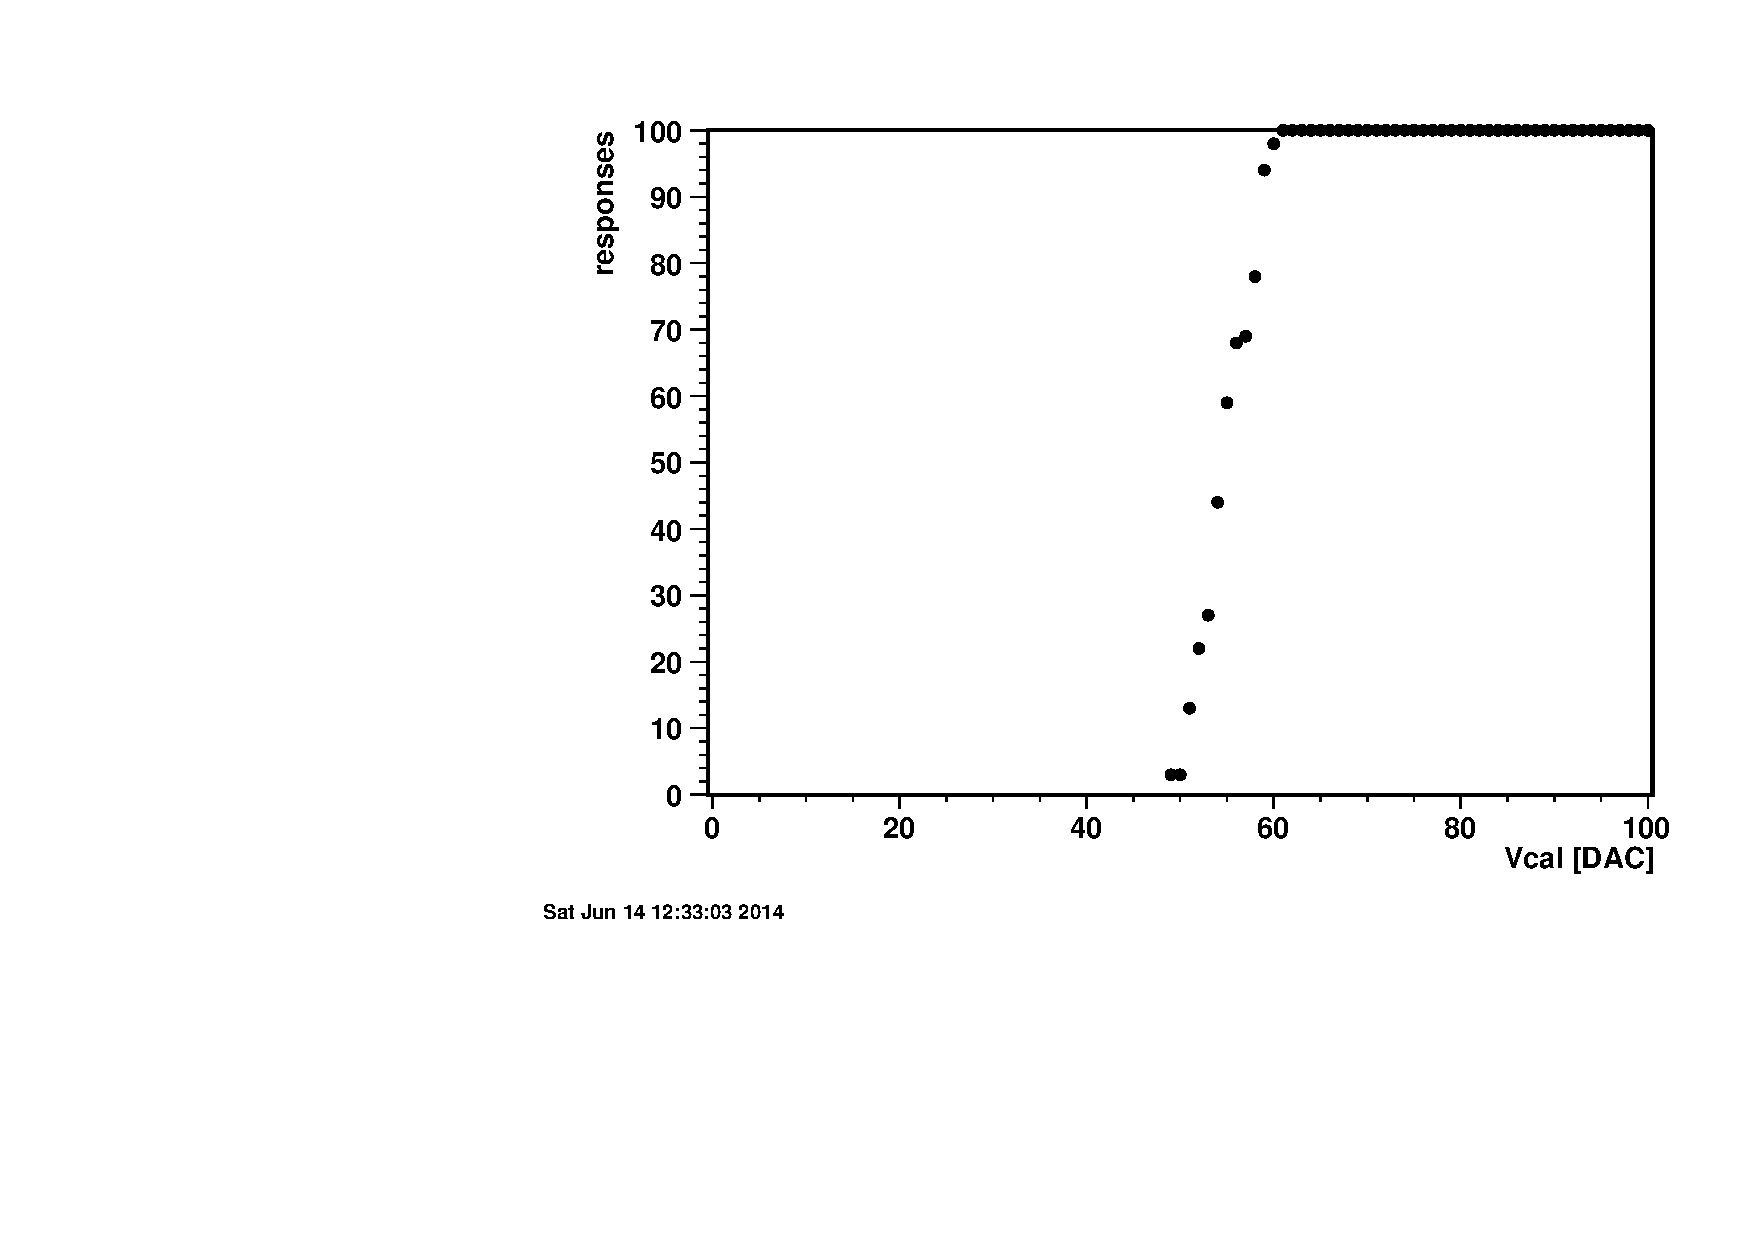
\includegraphics[scale=0.5]{c405-S-curve}\hfill{}~\protect\caption{Single pixel S-curve: counting responses to 100 triggers as a function
of the test pulse amplitude (in low range). The threshold is defined
as the Vcal value where 50\% efficiency is reached. The width of the
curve is taken as a measure of the noise.}
%
\end{figure}


%
\begin{figure}
\hfill{}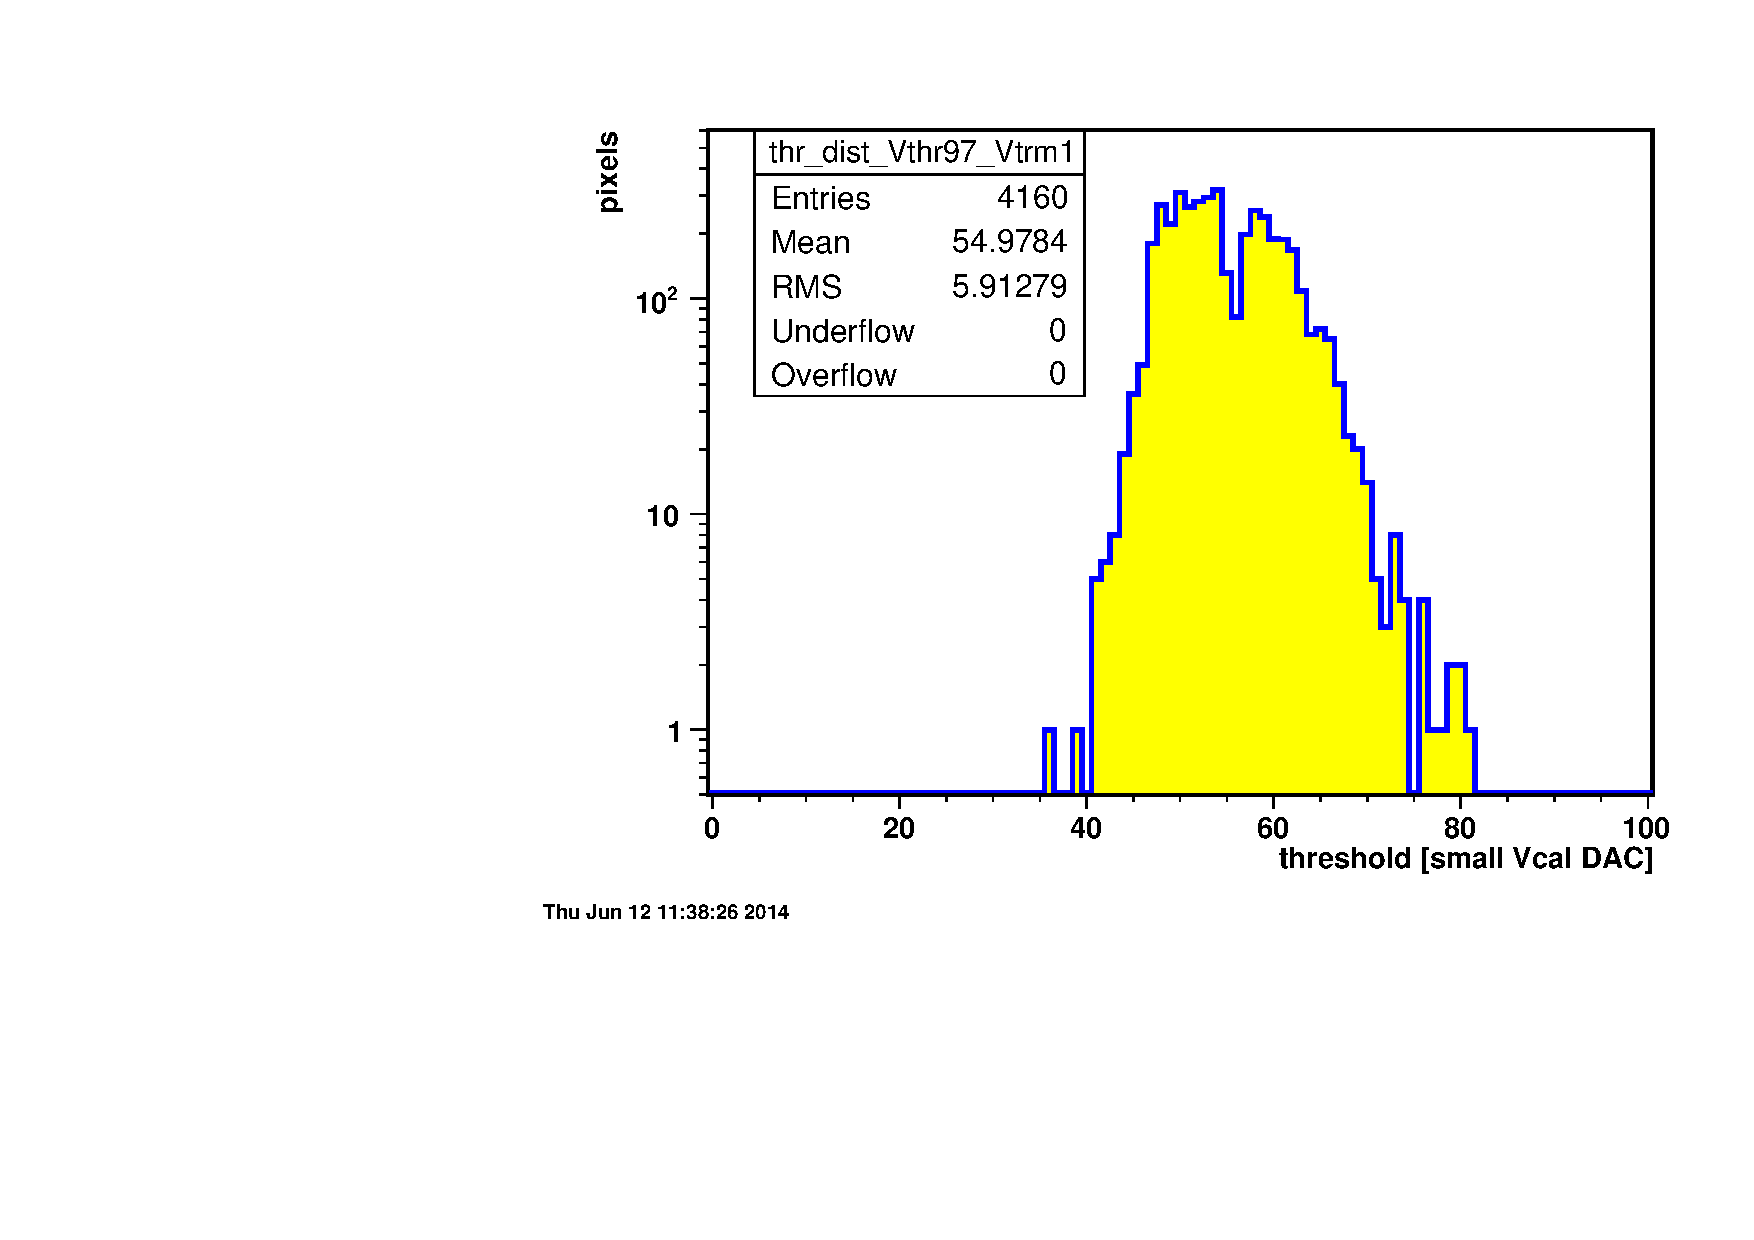
\includegraphics[scale=0.4]{c405-thrdist-untrimmed}\hfill{}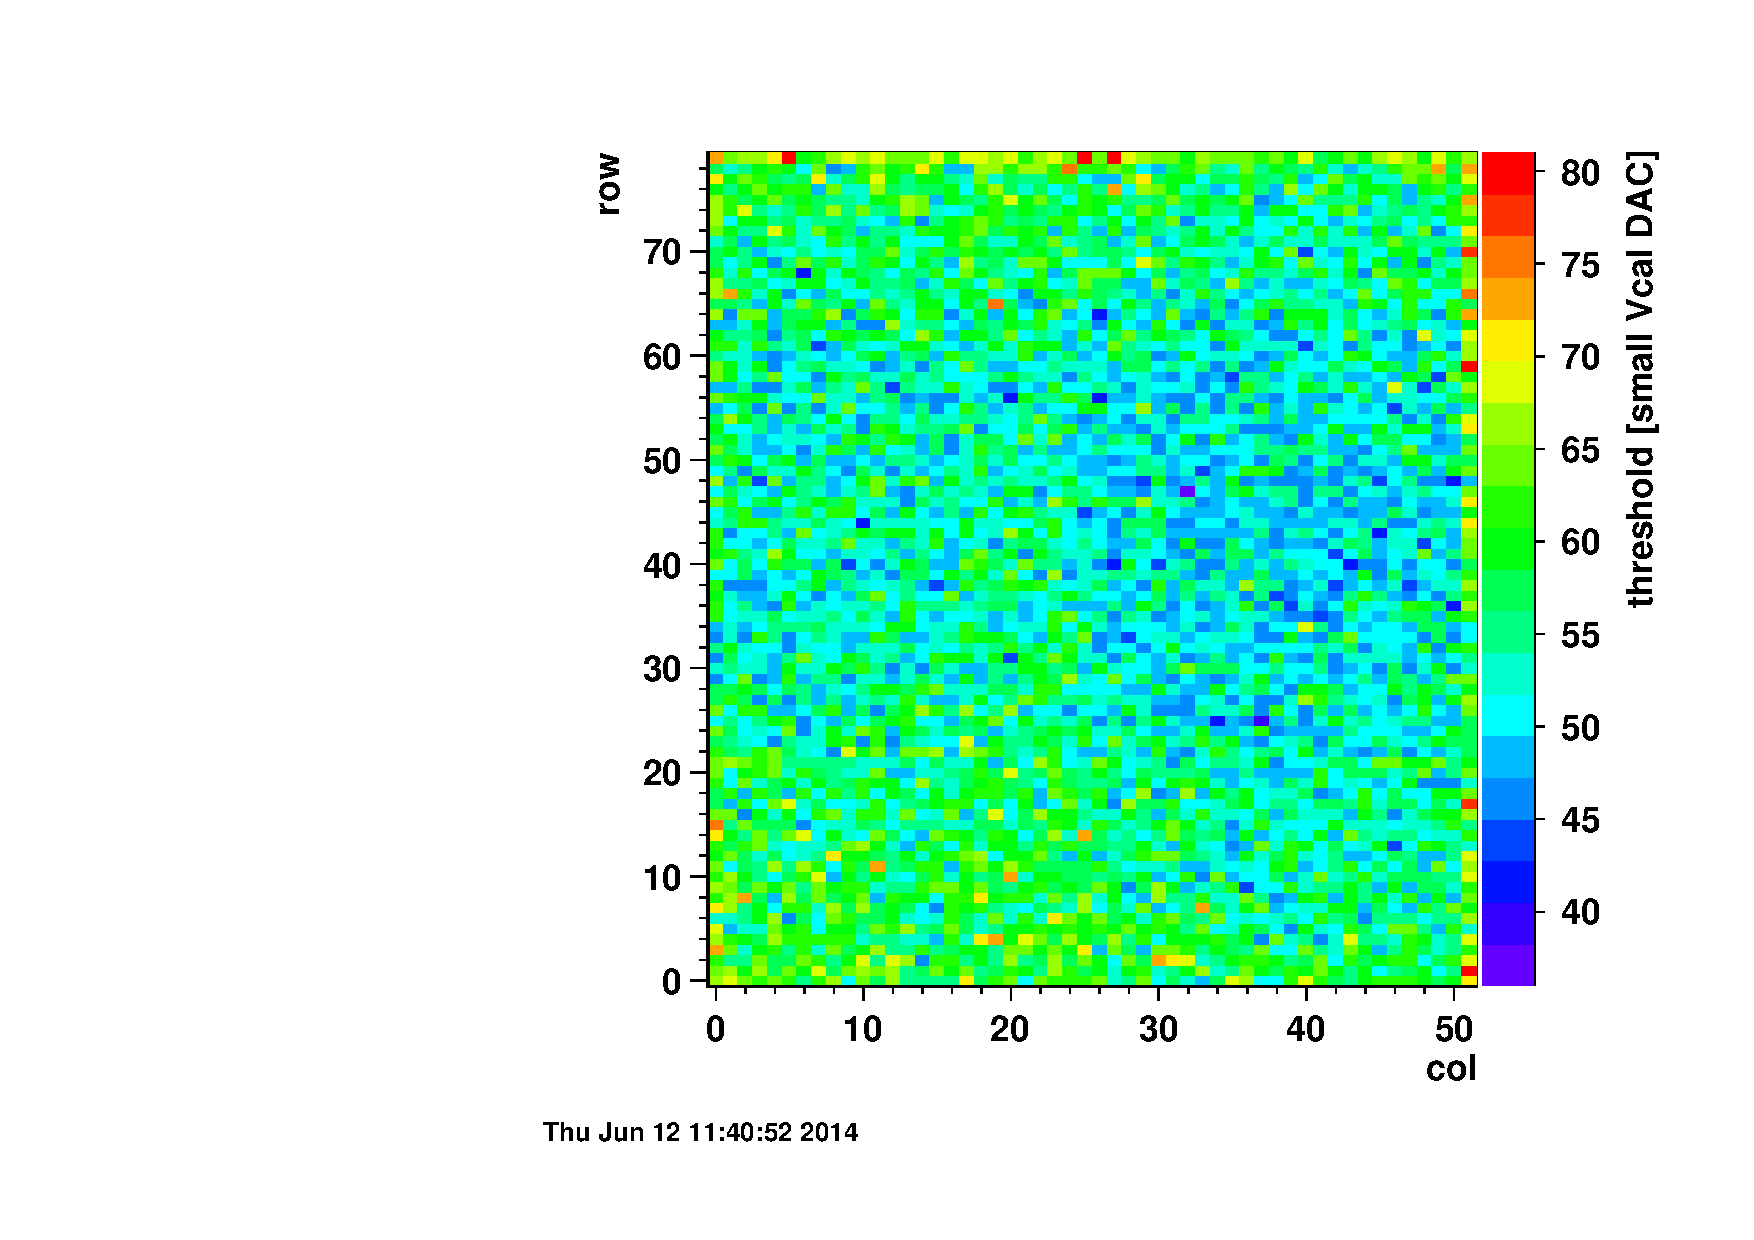
\includegraphics[scale=0.4]{c405-thrmap-untrimmed}\hfill{}~\protect\caption{threshold distribution and map, untrimmed digV2.1 chip}
%
\end{figure}


%
\begin{figure}
\hfill{}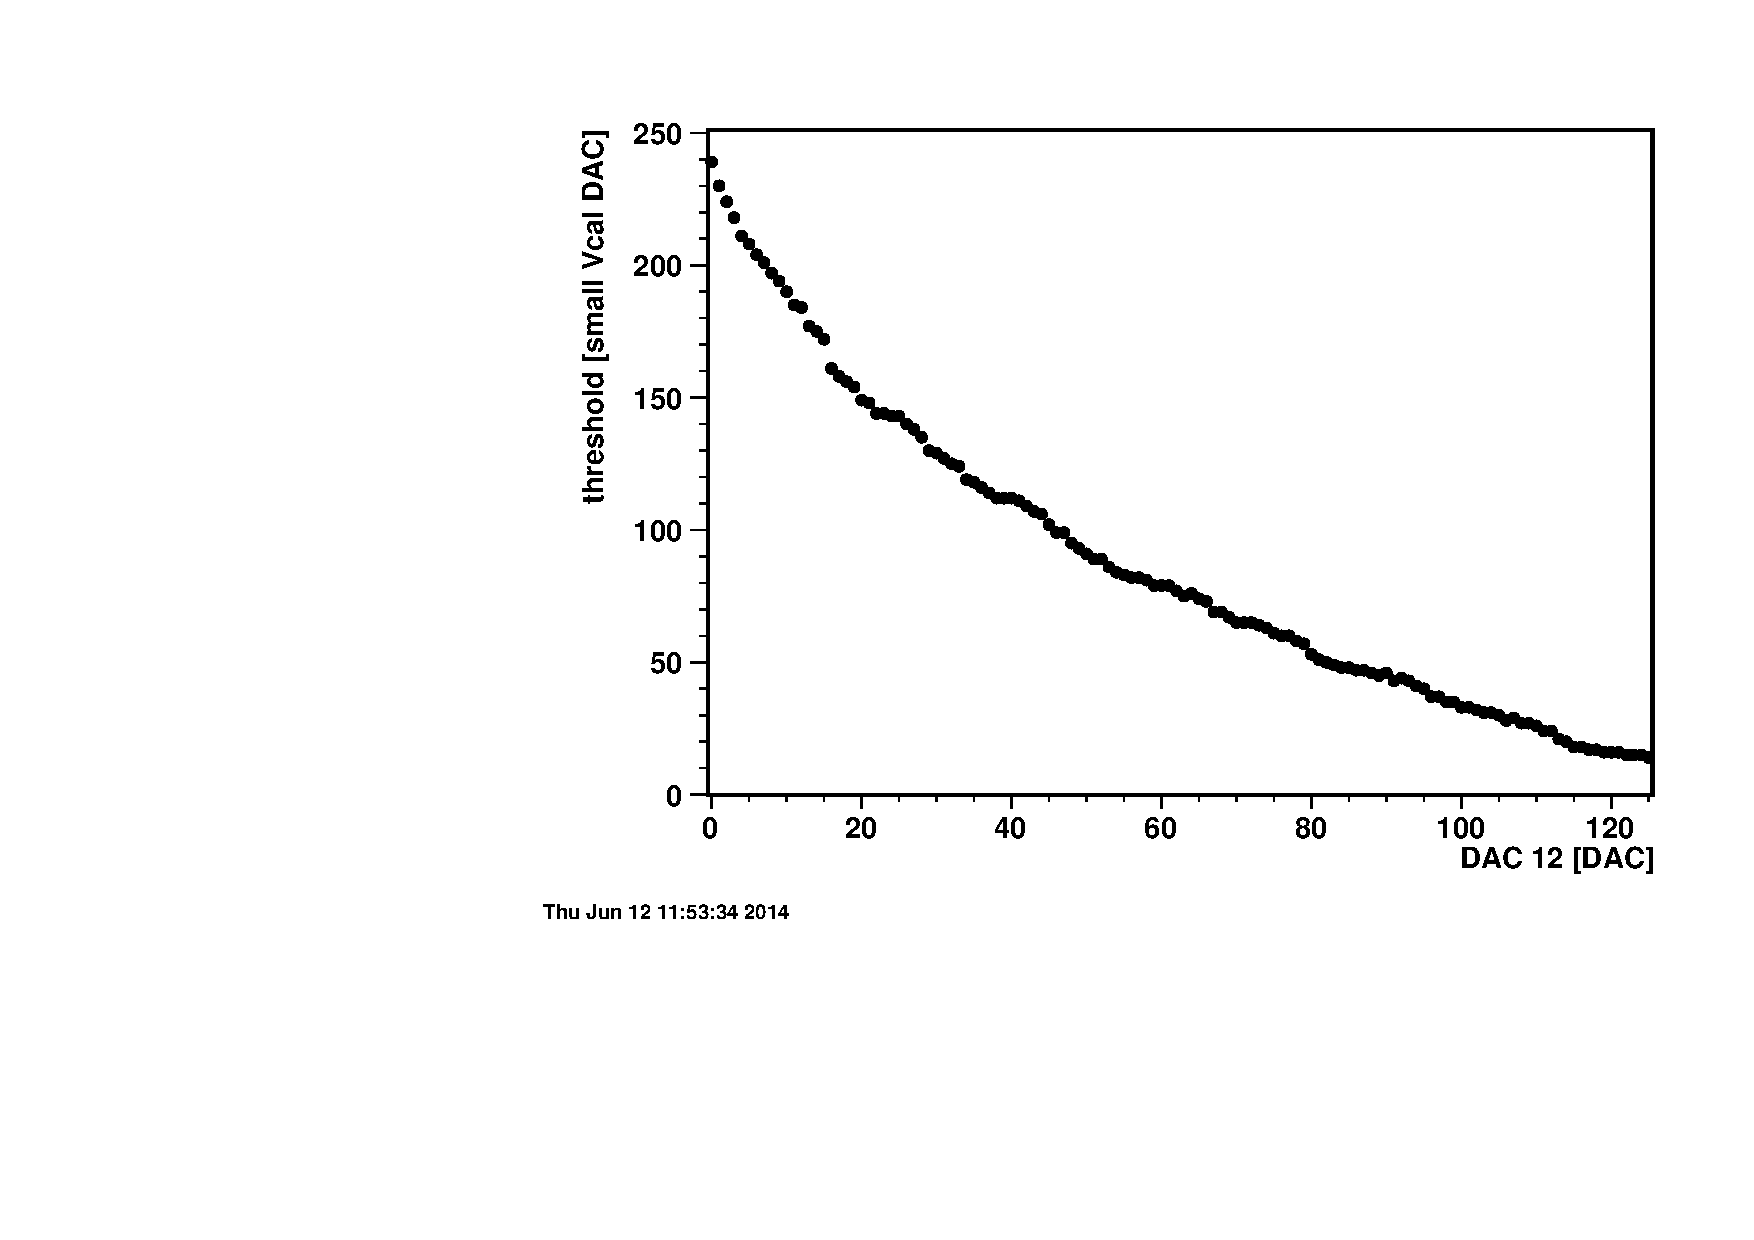
\includegraphics[scale=0.5]{c405-thr-vs-vthrcomp}\hfill{}~\protect\caption{pixel threshold vs global threshold}
%
\end{figure}


%
\begin{figure}
\hfill{}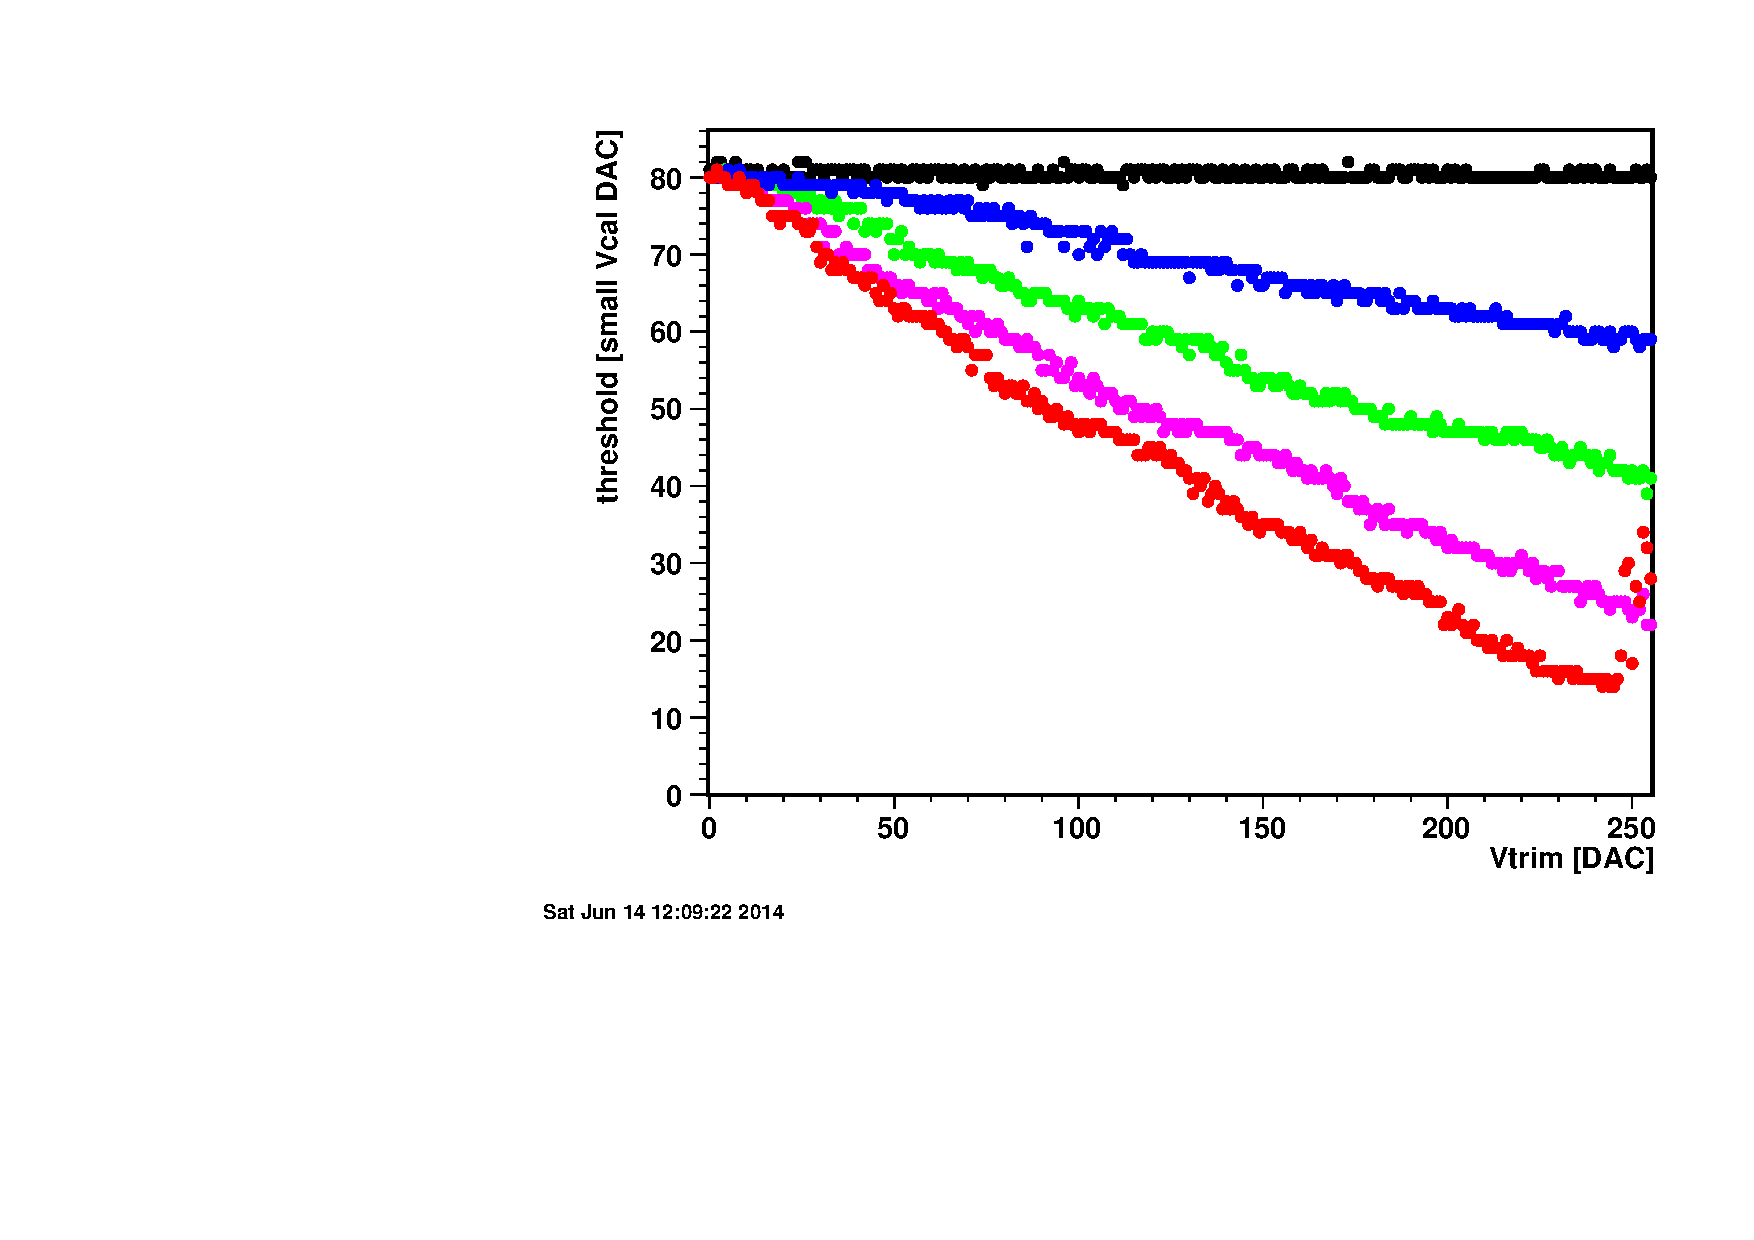
\includegraphics[scale=0.5]{c405-thr-vs-vtrim}\hfill{}~\protect\caption{Pixel threshold vs \texttt{Vtrim} for different \texttt{trim bits}:
top (black): 15, 2nd (blue): 11, mid (green): 7, 4th (magenta): 3,
bottom (red): 0 (at large \texttt{Vtrim} and and trim bits 0 the threshold
approaches the noise level and the measurement becomes unreliable).
The trim bit spacing is closer at smaller \texttt{Vtrim}, potentially
leading to a sharper threshold distribution.}
%
\end{figure}


%
\begin{figure}
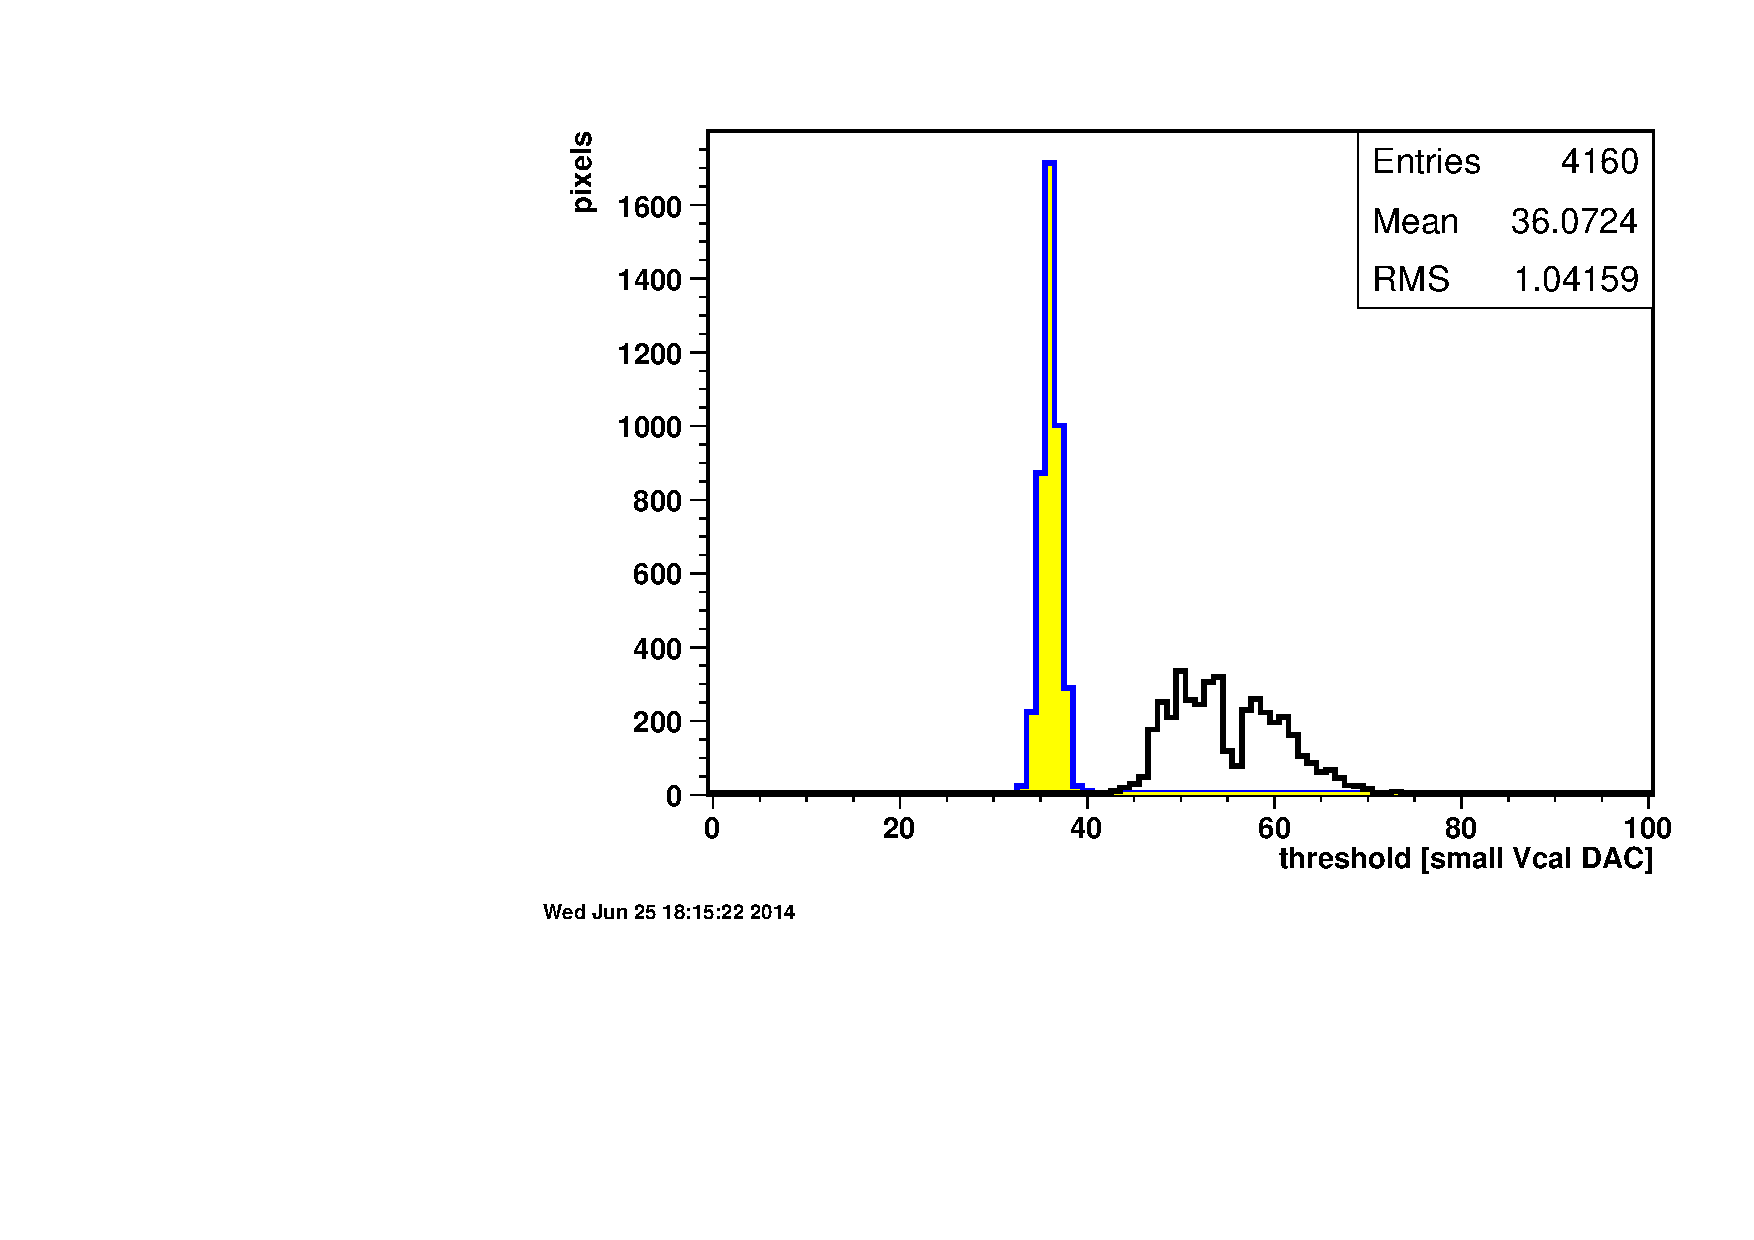
\includegraphics[scale=0.5]{c405-thrdist-trim36}\caption{threshold distribution before (black-white) and after trimming (blue-yellow).
The statistics box refers to the final distribution. 36 VcalDAC units
corresponds to about 1.8\,ke signal. The entire distribution can
still be shifted around using the global threshold \texttt{VthrComp}
while maintaining an RMS width of less than 2 DAC units.}
%
\end{figure}


%
\begin{figure}
\hfill{}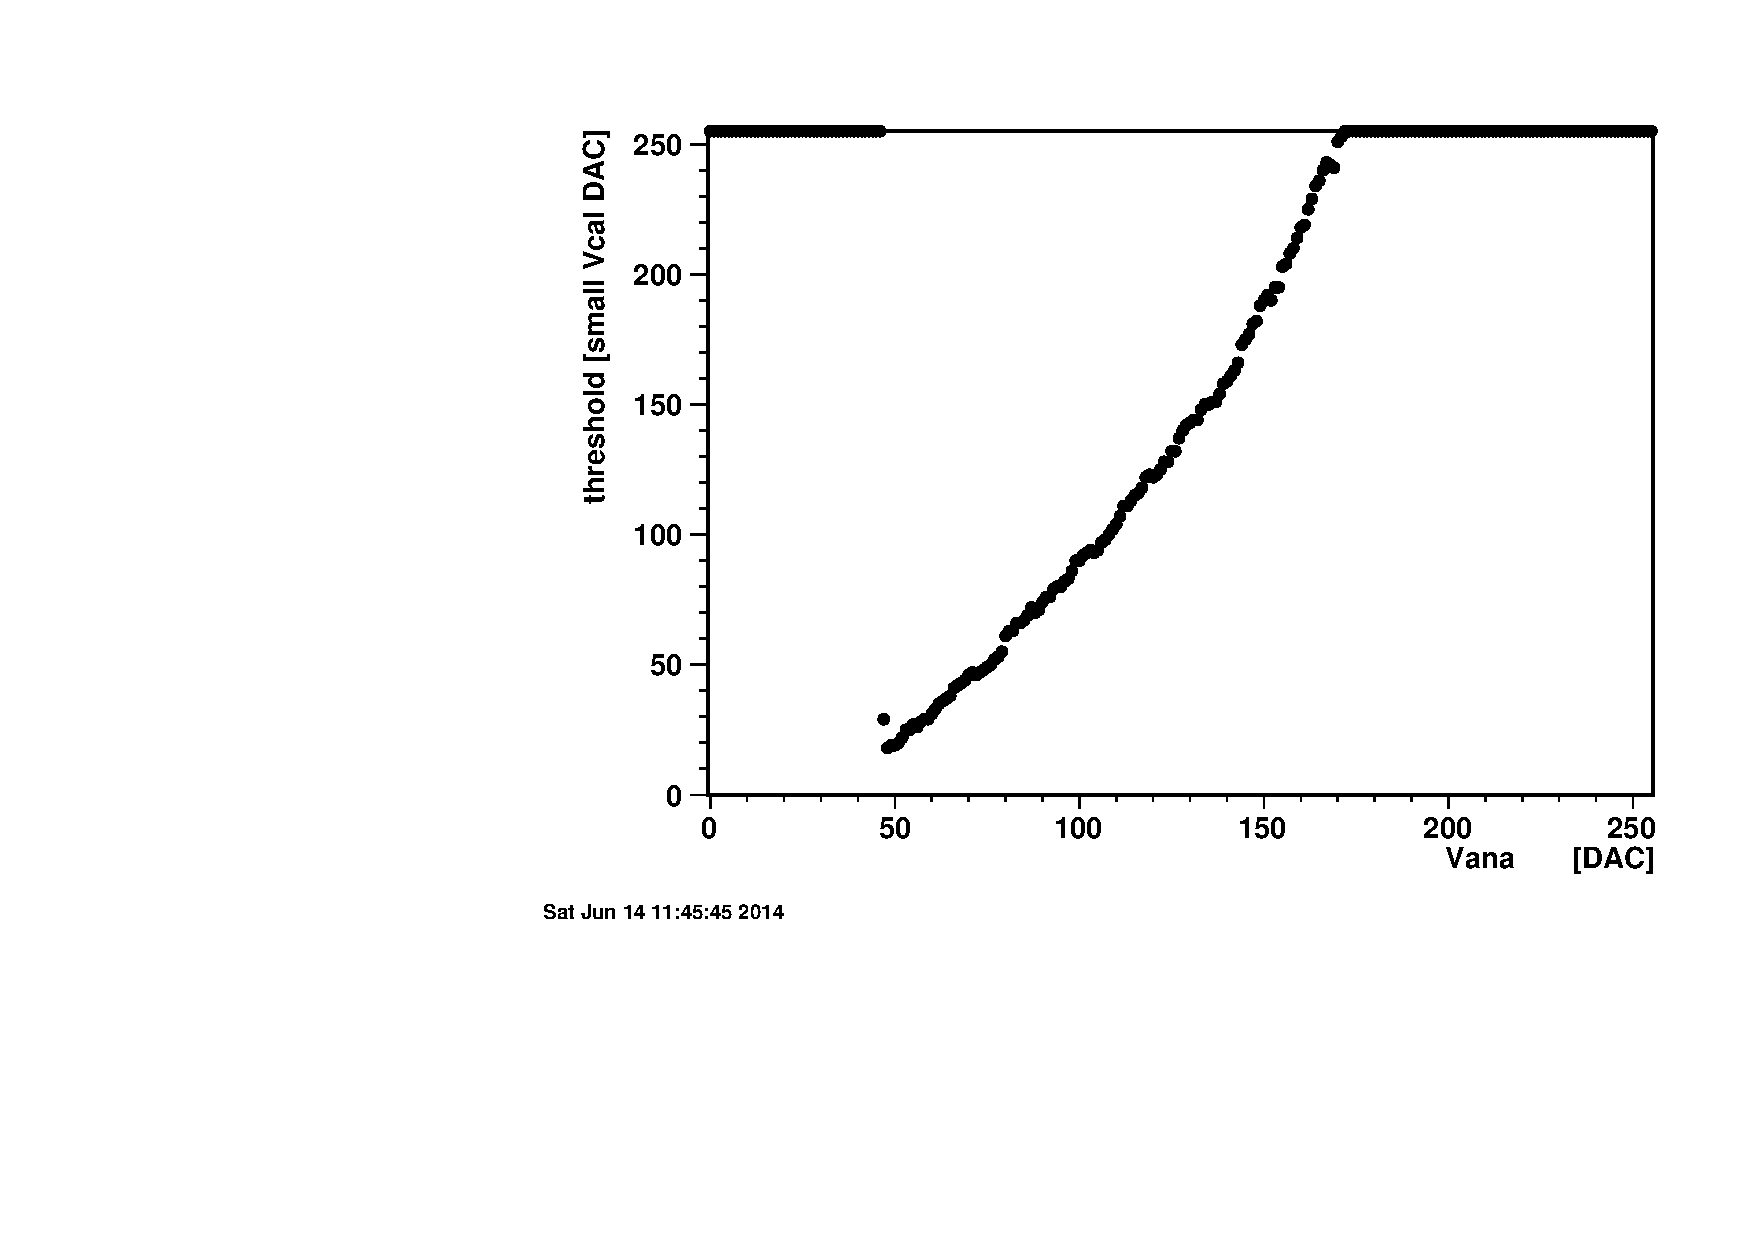
\includegraphics[scale=0.5]{c405-thr-vs-ia}\hfill{}~\protect\caption{Pixel threshold vs \texttt{Vana}. Threshold 255 means overflow (current
too low or threshold too high). Changing \texttt{Vana} changes the
working point of preamplifier and shaper and the baseline at the input
to the comparator, thus changing the pixel threshold with fixed comparator
settings (\texttt{VthrComp}, \texttt{Vtrim}). The order of setting
the DACs matters: don't change \texttt{Vana} after trimming (or re-trim,
or at least take a threshold map).}
%
\end{figure}


%
\begin{figure}
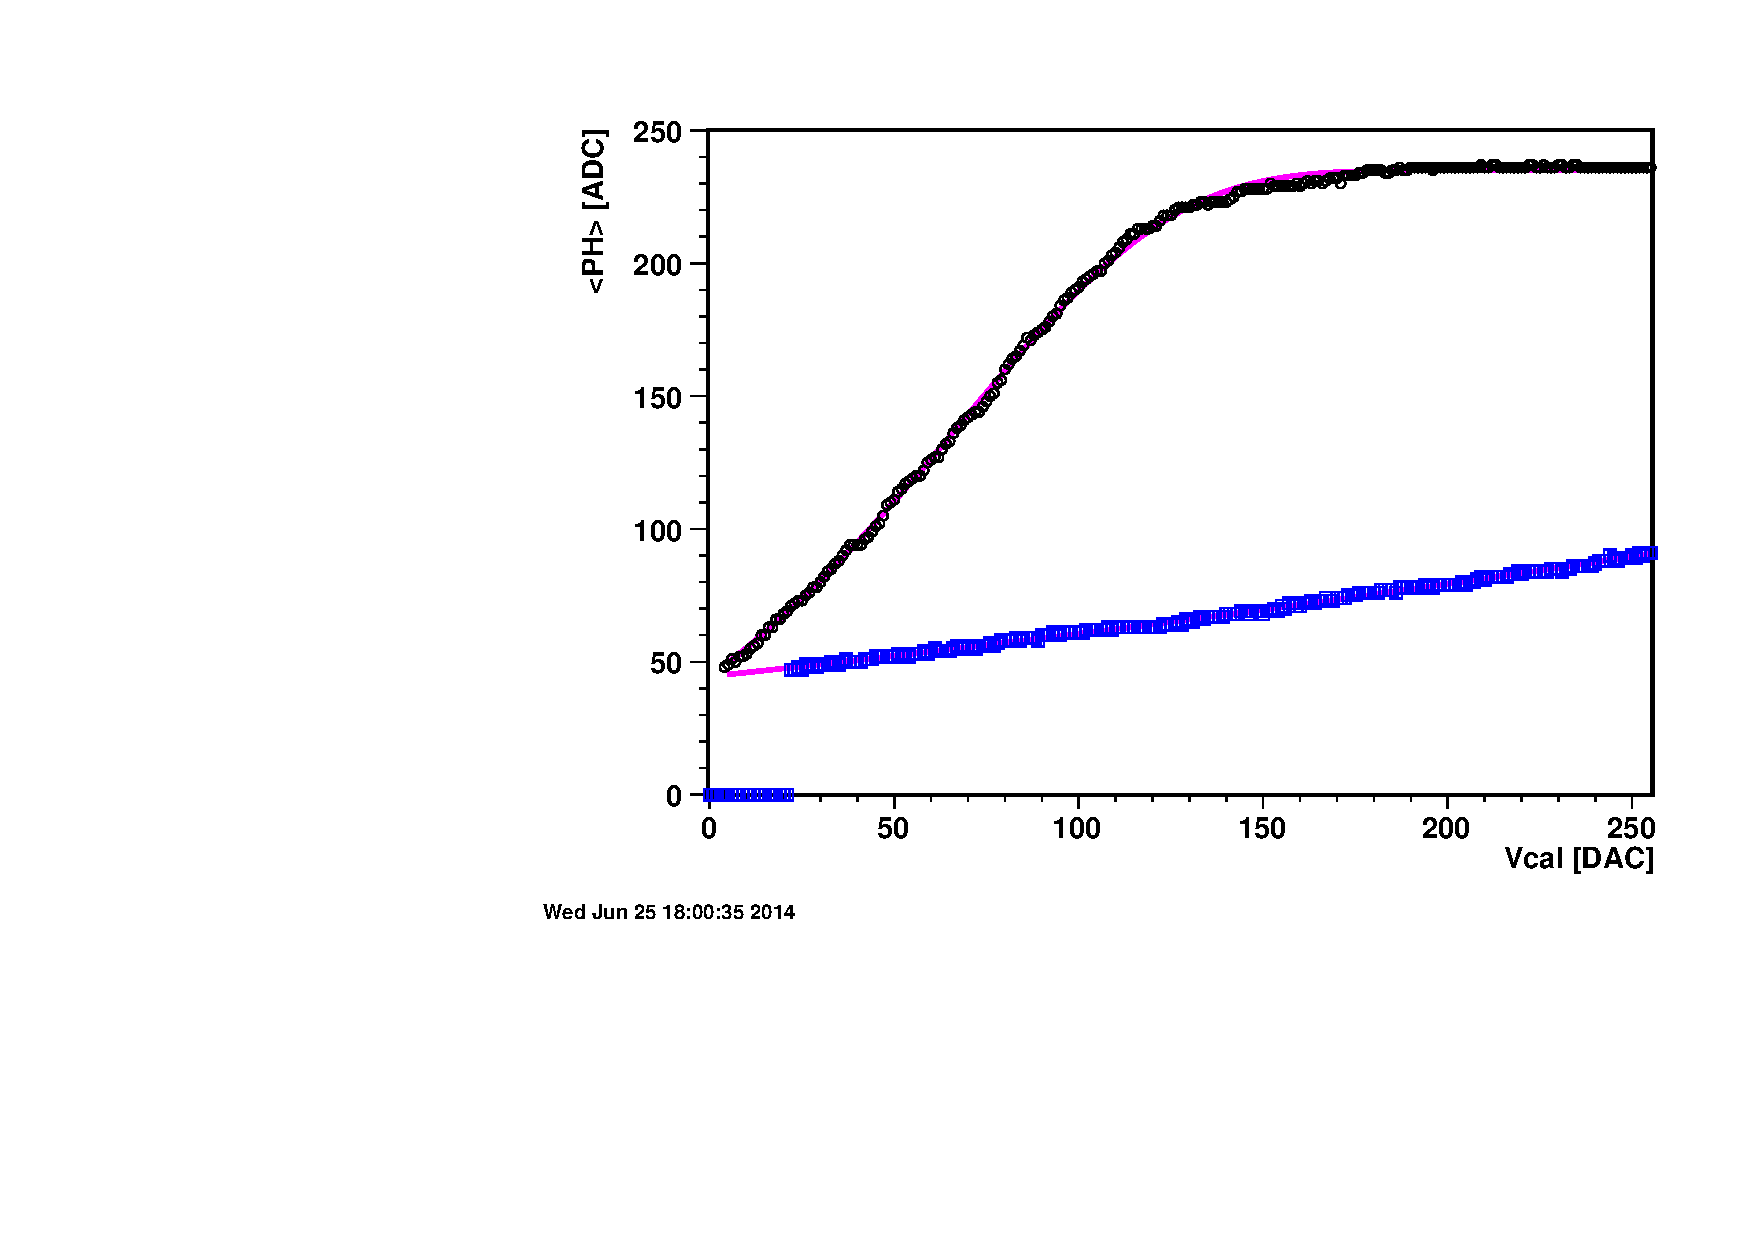
\includegraphics[scale=0.5]{PH-vs-Vcal-fit2}\caption{gain calibration: measure pulse height vs large (black) and small
(blue) Vcal and perform common fit to Weibull distribution (magenta).}
%
\end{figure}


%
\begin{figure}


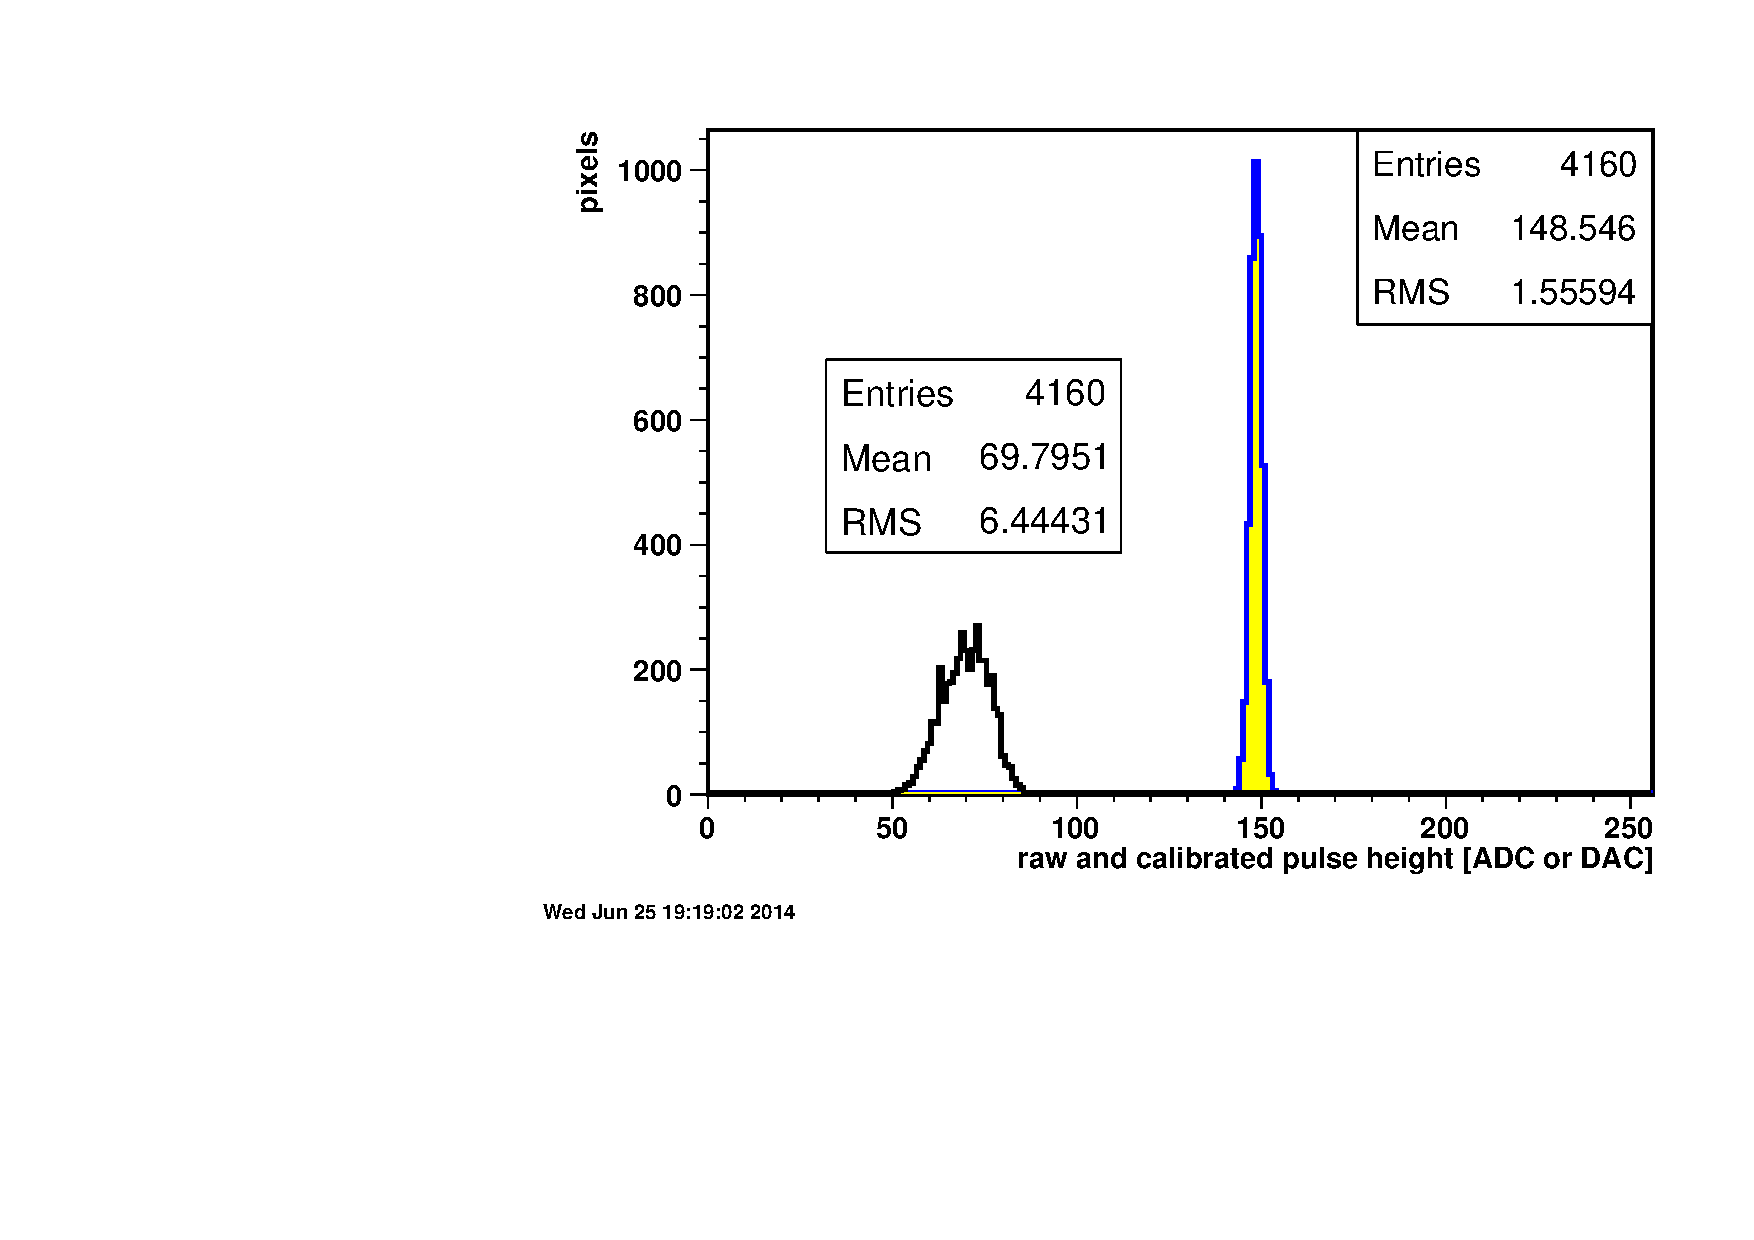
\includegraphics[scale=0.5]{c300-phdist}\caption{ROC pulse height distribution: raw ADC counts (black-white) and calibrated
Vcal DAC (blue-yellow)}
%
\end{figure}

\end{document}
